% Chapter 13: Speculative bubbles: LPPL models
% Time Series Analysis -- Bachelor's programmes Economic Informatics and Economic Cybernetics, Bucharest University of Economic Studies
% GENERATED by latex/build_chapter13.py -- edit the generator, not this file.

\newcommand{\coursename}{Time Series Analysis}
% Preambul comun TSA -- Serii de timp / Time Series Analysis (Beamer, 16:9)
% Același design ca MFM și SFM (preluat din SFM, 5 octombrie 2026). Înainte de % Preambul comun TSA -- Serii de timp / Time Series Analysis (Beamer, 16:9)
% Același design ca MFM și SFM (preluat din SFM, 5 octombrie 2026). Înainte de % Preambul comun TSA -- Serii de timp / Time Series Analysis (Beamer, 16:9)
% Același design ca MFM și SFM (preluat din SFM, 5 octombrie 2026). Înainte de \input{../../latex/preamble} se definește
%   \newcommand{\coursename}{Time Series Analysis}      (EN)
%   \newcommand{\coursename}{Serii de timp}       (RO)  și  \def\tsalang{ro}
% Fișierele .tex se află în EN/Courses, EN/Seminars, RO/Cursuri, RO/Seminarii (două niveluri sub rădăcină).
% Deck-urile sînt generate de latex/build_chapterN.py / build_seminarN.py (vezi latex/tsa_build.py).

\documentclass[9pt, aspectratio=169, t]{beamer}
\providecommand{\coursename}{Time Series Analysis}

% Ensure content fits on slides
\setbeamersize{text margin left=8mm, text margin right=8mm}
% Smaller institute font (title page)
\setbeamerfont{institute}{size=\footnotesize}

%=============================================================================
% THEME AND STYLE CONFIGURATION
%=============================================================================
\usetheme{default}
% Using default theme for clean header/footer control

% Color Palette (matching Redispatch PDF)
\definecolor{MainBlue}{RGB}{26, 58, 110}
\definecolor{AccentBlue}{RGB}{26, 58, 110}
\definecolor{IDAred}{RGB}{205, 0, 0}
\definecolor{DarkGray}{RGB}{51, 51, 51}
\definecolor{MediumGray}{RGB}{128, 128, 128}
\definecolor{LightGray}{RGB}{248, 248, 248}
\definecolor{VeryLightGray}{RGB}{235, 235, 235}
\definecolor{KeynoteGray}{RGB}{218, 218, 218}
\definecolor{SectionGray}{RGB}{120, 120, 120}
\definecolor{FooterGray}{RGB}{100, 100, 100}
\definecolor{Crimson}{RGB}{220, 53, 69}
\definecolor{Forest}{RGB}{46, 125, 50}
\definecolor{Amber}{RGB}{181, 133, 63}
\definecolor{Orange}{RGB}{230, 126, 34}
\definecolor{Purple}{RGB}{142, 68, 173}

% Gradient background (exact Keynote 315° gradient: white to RGB 218,218,218)
\setbeamertemplate{background}{%
    \begin{tikzpicture}[remember picture, overlay]
        \shade[shading=axis, shading angle=315,
        top color=white, bottom color=KeynoteGray]
        (current page.south west) rectangle (current page.north east);
    \end{tikzpicture}%
}
% Fallback solid color for compatibility
\setbeamercolor{background canvas}{bg=}

\setbeamercolor{palette primary}{bg=MainBlue, fg=white}
\setbeamercolor{palette secondary}{bg=MainBlue!85, fg=white}
\setbeamercolor{palette tertiary}{bg=MainBlue!70, fg=white}
\setbeamercolor{structure}{fg=MainBlue}
\setbeamercolor{title}{fg=IDAred}
\setbeamercolor{frametitle}{fg=IDAred, bg=}
\setbeamercolor{block title}{bg=MainBlue, fg=white}
\setbeamercolor{block body}{bg=VeryLightGray, fg=DarkGray}
\setbeamercolor{block title alerted}{bg=Crimson, fg=white}
\setbeamercolor{block body alerted}{bg=Crimson!8, fg=DarkGray}
\setbeamercolor{block title example}{bg=Forest, fg=white}
\setbeamercolor{block body example}{bg=Forest!8, fg=DarkGray}
\setbeamercolor{item}{fg=MainBlue}

% Footer colors (override Madrid theme blue)
\setbeamercolor{author in head/foot}{fg=FooterGray, bg=}
\setbeamercolor{title in head/foot}{fg=FooterGray, bg=}
\setbeamercolor{date in head/foot}{fg=FooterGray, bg=}
\setbeamercolor{section in head/foot}{fg=FooterGray, bg=}
\setbeamercolor{subsection in head/foot}{fg=FooterGray, bg=}

% Bullet styles (apply everywhere including blocks)
\setbeamertemplate{itemize item}{\color{MainBlue}$\boxdot$}
\setbeamertemplate{itemize subitem}{\color{MainBlue}$\blacktriangleright$}
\setbeamertemplate{itemize subsubitem}{\color{MainBlue}\tiny$\bullet$}
\setbeamertemplate{itemize/enumerate body begin}{\normalsize}
\setbeamertemplate{itemize/enumerate subbody begin}{\normalsize}

% Item spacing - compact style
\setlength{\leftmargini}{10pt}       % Level 1: minimal indent
\setlength{\leftmarginii}{10pt}      % Level 2: minimal additional indent
% Compact list spacing (zero extra space before/after lists in blocks)
\makeatletter
\def\@listi{\leftmargin\leftmargini \topsep 0pt \parsep 0pt \itemsep 0pt}
\def\@listii{\leftmargin\leftmarginii \topsep 0pt \parsep 0pt \itemsep 0pt}
\makeatother

\setbeamertemplate{navigation symbols}{}

%=============================================================================
% CUSTOM HEADLINE
%=============================================================================
\setbeamertemplate{headline}{%
    \vskip10pt%
    \hbox to \paperwidth{%
        \hskip0.5cm%
        {\small\color{FooterGray}\renewcommand{\hyperlink}[2]{##2}\insertsectionhead}%
        \hfill%
        \textcolor{FooterGray}{\small\insertframenumber}%
        \hskip0.5cm%
    }%
    \vskip4pt%
    {\color{FooterGray}\hrule height 0.4pt}%
}

%=============================================================================
% CUSTOM FOOTER
%=============================================================================
\usepackage{fontawesome5}

\setbeamertemplate{footline}{%
    {\color{FooterGray}\hrule height 0.4pt}%
    \vskip4pt%
    \hbox to \paperwidth{%
        \hskip0.5cm%
        \textcolor{FooterGray}{\small\coursename}%
        \hfill%
        \raisebox{-0.1em}{%
            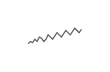
\begin{tikzpicture}[x=0.08em, y=0.08em, line width=0.4pt]
                \draw[FooterGray] (0,3) -- (1,4) -- (2,3.5) -- (3,5) -- (4,4) -- (5,6) -- (6,5.5) -- (7,4) -- (8,5) -- (9,7) -- (10,6) -- (11,5) -- (12,6.5) -- (13,8) -- (14,7) -- (15,6) -- (16,7.5) -- (17,9) -- (18,8) -- (19,7) -- (20,8.5) -- (21,10) -- (22,9) -- (23,8) -- (24,9.5);
            \end{tikzpicture}%
        }%
        \hskip0.5cm%
    }%
    \vskip6pt%
}

%=============================================================================
% PACKAGES
%=============================================================================
\usepackage[utf8]{inputenc}
\DeclareUnicodeCharacter{03B1}{\ensuremath{\alpha}}
\usepackage[T1]{fontenc}
\usepackage{amsmath, amssymb, amsthm}
\usepackage{mathtools}
\usepackage{bm}
\usepackage{tikz}
\usetikzlibrary{arrows.meta, positioning, shapes, calc, decorations.pathreplacing, shadings}
\usepackage{booktabs}
\usepackage{multirow}
\usepackage{array}
\usepackage{graphicx}
\usepackage{animate}
\usepackage{hyperref}
\usepackage{colortbl}
\usepackage{listings}
\lstset{language=Python, basicstyle=\ttfamily\scriptsize, keywordstyle=\color{MainBlue}\bfseries,
  commentstyle=\color{Forest}, stringstyle=\color{Crimson}, breaklines=true,
  frame=none, backgroundcolor=\color{VeryLightGray}, xleftmargin=2mm}
\hypersetup{colorlinks=true, linkcolor=MainBlue, urlcolor=MainBlue}
\graphicspath{{../../logos/}{../../charts/}{../../photos/}}
\usepackage{xcolor}
\hfuzz=2pt  % Suppress tiny overfull warnings (<2pt)
\vfuzz=2pt  % Suppress tiny vertical overfull warnings (<2pt)
% \mathrm in the sans-serif family of the slides (beamer resets \mathrm to the serif family at \begin{document};
% this hook runs after beamer's, so WN, Var, RMSE, ... in formulas match the surrounding text)
% Bold vectors and matrices in the same sans-serif family: \mathbf{A} in sans bold (beamer's own \mathbf came out in
% medium weight), and the bold upright Greek capitals of \boldsymbol / \bm (\bSigma, \bPhi, \boldsymbol{\Theta}) in
% cmss bold: bm.sty fixes its "boldoperators" font when it is loaded (serif cmbx), before beamer switches the
% operators to cmss, so it is reset here.
\AtBeginDocument{%
  \SetMathAlphabet{\mathrm}{normal}{\encodingdefault}{\sfdefault}{\mddefault}{n}%
  \SetMathAlphabet{\mathrm}{bold}{\encodingdefault}{\sfdefault}{bx}{n}%
  \SetMathAlphabet{\mathbf}{normal}{\encodingdefault}{\sfdefault}{bx}{n}%
  \SetMathAlphabet{\mathbf}{bold}{\encodingdefault}{\sfdefault}{bx}{n}%
  \SetSymbolFont{boldoperators}{normal}{OT1}{cmss}{bx}{n}%
  \SetSymbolFont{boldoperators}{bold}{OT1}{cmss}{bx}{n}}

%=============================================================================
% QUANTLET COMMANDS
%   \quantlet{<displayed name>}{<url>}       (generic, compatible with the older TSA decks)
%   \tsaquantlet{Ch_05}{TSA_ch5_garch}       -> https://github.com/danpele/Time-Series-Analysis/tree/main/Quantlets/Ch_05/TSA_ch5_garch
%   \qlurl{<folder>} is defined per chapter by the generator (Quantlets/Ch_NN/<folder>)
%=============================================================================
\newcommand{\tsarepo}{https://github.com/danpele/Time-Series-Analysis}
\newcommand{\tsaqlbase}{https://github.com/danpele/Time-Series-Analysis/tree/main/Quantlets}
\newcommand{\quantlet}[2]{%
    \hfill\href{#2}{%
        \raisebox{-0.15em}{
\includegraphics[height=0.7em]{ql_logo.png}}%
        \textcolor{MainBlue}{\tiny\ #1}%
    }%
}
\newcommand{\tsaquantlet}[2]{\quantlet{\detokenize{#2}}{\tsaqlbase/#1/#2}}

%=============================================================================
% NOTEBOOKS (Google Colab)
%   \colaburl{notebooks/EN/chapter5_seminar_notebook.ipynb} -> the Colab link of a file in the TSA repo
%   \nb: the chapter notebook (each seminar deck redefines it with \renewcommand)
%=============================================================================
\newcommand{\colaburl}[1]{https://colab.research.google.com/github/danpele/Time-Series-Analysis/blob/main/#1}
\newcommand{\nb}{https://colab.research.google.com/github/danpele/Time-Series-Analysis/tree/main/notebooks/EN}
\newcommand{\nbname}{notebooks/EN}

%=============================================================================
% SLIDE HELPERS (used by the generators; the same as in MFM)
%=============================================================================
% local font size for list bodies (the preamble forces \normalsize)
\newcommand{\itemsize}[1]{\setbeamertemplate{itemize/enumerate body begin}{#1}\setbeamertemplate{itemize/enumerate subbody begin}{#1}}
\newcommand{\intitle}[1]{{\hypersetup{urlcolor=white}#1}}   % white links inside coloured title bars
\newcommand{\imgcap}[1]{{\scriptsize #1}\\[0.5mm]}          % caption under a photo
\newcommand{\imgcredit}[2]{{\tiny\color{FooterGray}\href{#1}{#2}}}   % image credit: source URL, author/licence
\newcommand{\aiprompt}[1]{{\ttfamily\color{MainBlue}#1}}     % a prompt to an AI assistant

%=============================================================================
% SEMINARS: student version by default; the instructor wrapper *_solutions.tex sets \solutionstrue
%=============================================================================
\makeatletter\@ifundefined{ifsolutions}{\expandafter\newif\csname ifsolutions\endcsname}{}\makeatother
\newcommand{\solonly}[1]{\ifsolutions #1\fi}
\newcommand{\propsub}{\ifsolutions\else\framesubtitle{\ifdefined\tsalang Rezolvarea se discută la seminar\else Solution discussed in class\fi}\fi}

%=============================================================================
% APPENDIX AND CHAPTER LINKS (latex/appendix_links.py writes the calls; it also re-declares these
% macros before \begin{document}, so the decks compile with or without this preamble block)
%=============================================================================
\providecommand{\tsaapplink}[3]{\hypertarget{#2}{}\hyperlink{#1}{\beamergotobutton{#3}}}
\providecommand{\tsaappback}[2]{\begin{tikzpicture}[remember picture,overlay]\node[anchor=south east] at ([xshift=-3mm,yshift=7mm]current page.south east){\hyperlink{#1}{\beamerreturnbutton{#2}}};\end{tikzpicture}}
\providecommand{\tsachlink}[2]{\href{#1}{#2}}
\providecommand{\tsachlinkt}[2]{\href{#1}{\usebeamercolor[fg]{frametitle}#2}}

%=============================================================================
% QUANTINAR COMMAND: link către un curs Quantinar (subiecte avansate)
%=============================================================================
\newcommand{\quantinar}[2]{%
    \href{#2}{%
        \raisebox{-0.15em}{
\includegraphics[height=0.8em]{qr_logo.png}}%
        \textcolor{MainBlue}{\scriptsize\ #1}%
    }%
}

%=============================================================================
% CUSTOM TITLE PAGE
%=============================================================================
\defbeamertemplate*{title page}{hybrid}[1][]
{
    \vspace{0.2cm}
    % Logos row - top header (with clickable links)
    \begin{center}
        \href{https://www.ase.ro}{
\includegraphics[height=1.0cm]{ase_logo.png}}\hspace{0.3cm}%
        \href{https://theida.net}{
\includegraphics[height=1.0cm]{ida_logo.png}}\hspace{0.3cm}%
        \href{https://blockchain-research-center.com}{
\includegraphics[height=1.0cm]{brc_logo.png}}\hspace{0.3cm}%
        \href{https://www.ai4efin.ase.ro}{
\includegraphics[height=1.0cm]{ai4efin_logo.png}}\hspace{0.3cm}%
        \href{https://ipe.ro/new}{
\includegraphics[height=1.0cm]{acad_logo.png}}\hspace{0.3cm}%
        \href{https://www.digital-finance-msca.com}{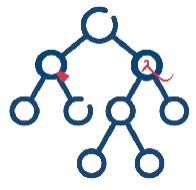
\includegraphics[height=1.0cm]{msca_logo.png}}%
    \end{center}

    \vspace{0.6cm}

    % Main title with Q logos on sides (with clickable links)
    \begin{center}
        \begin{minipage}{0.1\textwidth}
            \centering
            \href{https://quantlet.com}{
\includegraphics[height=1.1cm]{ql_logo.png}}
        \end{minipage}%
        \begin{minipage}{0.78\textwidth}
            \centering
            {\LARGE\bfseries\usebeamercolor[fg]{title}\inserttitle}

            \vspace{0.3cm}

            {\usebeamerfont{subtitle}\usebeamercolor[fg]{title}\insertsubtitle}
        \end{minipage}%
        \begin{minipage}{0.1\textwidth}
            \centering
            \href{https://quantinar.com}{
\includegraphics[height=1.1cm]{qr_logo.png}}
        \end{minipage}
    \end{center}

    \vspace{0.6cm}

    % Authors (left aligned)
    \hspace{0.5cm}{\usebeamerfont{author}\insertauthor}

    \vspace{0.3cm}

    % Institute/Affiliations (left aligned)
    \hspace{0.5cm}\begin{minipage}[t]{0.9\textwidth}
        \raggedright\small\insertinstitute
    \end{minipage}
}

%=============================================================================
% THEOREM ENVIRONMENTS
%=============================================================================
\theoremstyle{definition}
\setbeamertemplate{theorems}[numbered]
\ifdefined\tsalang
\newtheorem{defn}{Definiție}
\newtheorem{thm}{Teoremă}
\newtheorem{prop}{Propoziție}
\newtheorem{rmk}{Observație}
\else
\newtheorem{defn}{Definition}
\newtheorem{thm}{Theorem}
\newtheorem{prop}{Proposition}
\newtheorem{rmk}{Remark}
\fi

%=============================================================================
% CENTRED MINIPAGE (no extra vertical space)
%=============================================================================
\newenvironment{cminipage}[1]{%
    \par\noindent\hfill\begin{minipage}{#1}\ignorespaces
}{%
    \end{minipage}\hfill\null\par
}

%=============================================================================
% CUSTOM COMMANDS
%=============================================================================
\newcommand{\E}{\mathbb{E}}
\newcommand{\Var}{\text{Var}}
\newcommand{\Cov}{\text{Cov}}
\newcommand{\Corr}{\text{Corr}}
\newcommand{\R}{\mathbb{R}}
\newcommand{\N}{\mathbb{N}}
\newcommand{\Z}{\mathbb{Z}}
\newcommand{\B}{\mathbf{B}}
\newcommand{\imark}{\textcolor{MainBlue}{\textbullet}}
\newcommand{\RMSE}{\text{RMSE}}
\newcommand{\MAE}{\text{MAE}}
\newcommand{\MAPE}{\text{MAPE}}

% Boldface vector/matrix commands (VAR, VECM, state space; also used by the older TSA decks)
\newcommand{\bY}{\mathbf{Y}}
\newcommand{\bX}{\mathbf{X}}
\newcommand{\bA}{\mathbf{A}}
\newcommand{\bB}{\mathbf{B}}
\newcommand{\bepsilon}{\boldsymbol{\varepsilon}}
\newcommand{\bSigma}{\boldsymbol{\Sigma}}
\newcommand{\bPhi}{\boldsymbol{\Phi}}
\newcommand{\bGamma}{\boldsymbol{\Gamma}}
\newcommand{\bPi}{\boldsymbol{\Pi}}
\newcommand{\bc}{\mathbf{c}}
\newcommand{\balpha}{\boldsymbol{\alpha}}
\newcommand{\bbeta}{\boldsymbol{\beta}}
\newcommand{\bvarepsilon}{\boldsymbol{\varepsilon}}

% Legacy seminar marks (older TSA seminar decks)
\newcommand{\correct}{\textcolor{Forest}{\checkmark}}
\newcommand{\incorrect}{\textcolor{Crimson}{\texttimes}}
 se definește
%   \newcommand{\coursename}{Time Series Analysis}      (EN)
%   \newcommand{\coursename}{Serii de timp}       (RO)  și  \def\tsalang{ro}
% Fișierele .tex se află în EN/Courses, EN/Seminars, RO/Cursuri, RO/Seminarii (două niveluri sub rădăcină).
% Deck-urile sînt generate de latex/build_chapterN.py / build_seminarN.py (vezi latex/tsa_build.py).

\documentclass[9pt, aspectratio=169, t]{beamer}
\providecommand{\coursename}{Time Series Analysis}

% Ensure content fits on slides
\setbeamersize{text margin left=8mm, text margin right=8mm}
% Smaller institute font (title page)
\setbeamerfont{institute}{size=\footnotesize}

%=============================================================================
% THEME AND STYLE CONFIGURATION
%=============================================================================
\usetheme{default}
% Using default theme for clean header/footer control

% Color Palette (matching Redispatch PDF)
\definecolor{MainBlue}{RGB}{26, 58, 110}
\definecolor{AccentBlue}{RGB}{26, 58, 110}
\definecolor{IDAred}{RGB}{205, 0, 0}
\definecolor{DarkGray}{RGB}{51, 51, 51}
\definecolor{MediumGray}{RGB}{128, 128, 128}
\definecolor{LightGray}{RGB}{248, 248, 248}
\definecolor{VeryLightGray}{RGB}{235, 235, 235}
\definecolor{KeynoteGray}{RGB}{218, 218, 218}
\definecolor{SectionGray}{RGB}{120, 120, 120}
\definecolor{FooterGray}{RGB}{100, 100, 100}
\definecolor{Crimson}{RGB}{220, 53, 69}
\definecolor{Forest}{RGB}{46, 125, 50}
\definecolor{Amber}{RGB}{181, 133, 63}
\definecolor{Orange}{RGB}{230, 126, 34}
\definecolor{Purple}{RGB}{142, 68, 173}

% Gradient background (exact Keynote 315° gradient: white to RGB 218,218,218)
\setbeamertemplate{background}{%
    \begin{tikzpicture}[remember picture, overlay]
        \shade[shading=axis, shading angle=315,
        top color=white, bottom color=KeynoteGray]
        (current page.south west) rectangle (current page.north east);
    \end{tikzpicture}%
}
% Fallback solid color for compatibility
\setbeamercolor{background canvas}{bg=}

\setbeamercolor{palette primary}{bg=MainBlue, fg=white}
\setbeamercolor{palette secondary}{bg=MainBlue!85, fg=white}
\setbeamercolor{palette tertiary}{bg=MainBlue!70, fg=white}
\setbeamercolor{structure}{fg=MainBlue}
\setbeamercolor{title}{fg=IDAred}
\setbeamercolor{frametitle}{fg=IDAred, bg=}
\setbeamercolor{block title}{bg=MainBlue, fg=white}
\setbeamercolor{block body}{bg=VeryLightGray, fg=DarkGray}
\setbeamercolor{block title alerted}{bg=Crimson, fg=white}
\setbeamercolor{block body alerted}{bg=Crimson!8, fg=DarkGray}
\setbeamercolor{block title example}{bg=Forest, fg=white}
\setbeamercolor{block body example}{bg=Forest!8, fg=DarkGray}
\setbeamercolor{item}{fg=MainBlue}

% Footer colors (override Madrid theme blue)
\setbeamercolor{author in head/foot}{fg=FooterGray, bg=}
\setbeamercolor{title in head/foot}{fg=FooterGray, bg=}
\setbeamercolor{date in head/foot}{fg=FooterGray, bg=}
\setbeamercolor{section in head/foot}{fg=FooterGray, bg=}
\setbeamercolor{subsection in head/foot}{fg=FooterGray, bg=}

% Bullet styles (apply everywhere including blocks)
\setbeamertemplate{itemize item}{\color{MainBlue}$\boxdot$}
\setbeamertemplate{itemize subitem}{\color{MainBlue}$\blacktriangleright$}
\setbeamertemplate{itemize subsubitem}{\color{MainBlue}\tiny$\bullet$}
\setbeamertemplate{itemize/enumerate body begin}{\normalsize}
\setbeamertemplate{itemize/enumerate subbody begin}{\normalsize}

% Item spacing - compact style
\setlength{\leftmargini}{10pt}       % Level 1: minimal indent
\setlength{\leftmarginii}{10pt}      % Level 2: minimal additional indent
% Compact list spacing (zero extra space before/after lists in blocks)
\makeatletter
\def\@listi{\leftmargin\leftmargini \topsep 0pt \parsep 0pt \itemsep 0pt}
\def\@listii{\leftmargin\leftmarginii \topsep 0pt \parsep 0pt \itemsep 0pt}
\makeatother

\setbeamertemplate{navigation symbols}{}

%=============================================================================
% CUSTOM HEADLINE
%=============================================================================
\setbeamertemplate{headline}{%
    \vskip10pt%
    \hbox to \paperwidth{%
        \hskip0.5cm%
        {\small\color{FooterGray}\renewcommand{\hyperlink}[2]{##2}\insertsectionhead}%
        \hfill%
        \textcolor{FooterGray}{\small\insertframenumber}%
        \hskip0.5cm%
    }%
    \vskip4pt%
    {\color{FooterGray}\hrule height 0.4pt}%
}

%=============================================================================
% CUSTOM FOOTER
%=============================================================================
\usepackage{fontawesome5}

\setbeamertemplate{footline}{%
    {\color{FooterGray}\hrule height 0.4pt}%
    \vskip4pt%
    \hbox to \paperwidth{%
        \hskip0.5cm%
        \textcolor{FooterGray}{\small\coursename}%
        \hfill%
        \raisebox{-0.1em}{%
            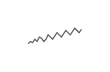
\begin{tikzpicture}[x=0.08em, y=0.08em, line width=0.4pt]
                \draw[FooterGray] (0,3) -- (1,4) -- (2,3.5) -- (3,5) -- (4,4) -- (5,6) -- (6,5.5) -- (7,4) -- (8,5) -- (9,7) -- (10,6) -- (11,5) -- (12,6.5) -- (13,8) -- (14,7) -- (15,6) -- (16,7.5) -- (17,9) -- (18,8) -- (19,7) -- (20,8.5) -- (21,10) -- (22,9) -- (23,8) -- (24,9.5);
            \end{tikzpicture}%
        }%
        \hskip0.5cm%
    }%
    \vskip6pt%
}

%=============================================================================
% PACKAGES
%=============================================================================
\usepackage[utf8]{inputenc}
\DeclareUnicodeCharacter{03B1}{\ensuremath{\alpha}}
\usepackage[T1]{fontenc}
\usepackage{amsmath, amssymb, amsthm}
\usepackage{mathtools}
\usepackage{bm}
\usepackage{tikz}
\usetikzlibrary{arrows.meta, positioning, shapes, calc, decorations.pathreplacing, shadings}
\usepackage{booktabs}
\usepackage{multirow}
\usepackage{array}
\usepackage{graphicx}
\usepackage{animate}
\usepackage{hyperref}
\usepackage{colortbl}
\usepackage{listings}
\lstset{language=Python, basicstyle=\ttfamily\scriptsize, keywordstyle=\color{MainBlue}\bfseries,
  commentstyle=\color{Forest}, stringstyle=\color{Crimson}, breaklines=true,
  frame=none, backgroundcolor=\color{VeryLightGray}, xleftmargin=2mm}
\hypersetup{colorlinks=true, linkcolor=MainBlue, urlcolor=MainBlue}
\graphicspath{{../../logos/}{../../charts/}{../../photos/}}
\usepackage{xcolor}
\hfuzz=2pt  % Suppress tiny overfull warnings (<2pt)
\vfuzz=2pt  % Suppress tiny vertical overfull warnings (<2pt)
% \mathrm in the sans-serif family of the slides (beamer resets \mathrm to the serif family at \begin{document};
% this hook runs after beamer's, so WN, Var, RMSE, ... in formulas match the surrounding text)
% Bold vectors and matrices in the same sans-serif family: \mathbf{A} in sans bold (beamer's own \mathbf came out in
% medium weight), and the bold upright Greek capitals of \boldsymbol / \bm (\bSigma, \bPhi, \boldsymbol{\Theta}) in
% cmss bold: bm.sty fixes its "boldoperators" font when it is loaded (serif cmbx), before beamer switches the
% operators to cmss, so it is reset here.
\AtBeginDocument{%
  \SetMathAlphabet{\mathrm}{normal}{\encodingdefault}{\sfdefault}{\mddefault}{n}%
  \SetMathAlphabet{\mathrm}{bold}{\encodingdefault}{\sfdefault}{bx}{n}%
  \SetMathAlphabet{\mathbf}{normal}{\encodingdefault}{\sfdefault}{bx}{n}%
  \SetMathAlphabet{\mathbf}{bold}{\encodingdefault}{\sfdefault}{bx}{n}%
  \SetSymbolFont{boldoperators}{normal}{OT1}{cmss}{bx}{n}%
  \SetSymbolFont{boldoperators}{bold}{OT1}{cmss}{bx}{n}}

%=============================================================================
% QUANTLET COMMANDS
%   \quantlet{<displayed name>}{<url>}       (generic, compatible with the older TSA decks)
%   \tsaquantlet{Ch_05}{TSA_ch5_garch}       -> https://github.com/danpele/Time-Series-Analysis/tree/main/Quantlets/Ch_05/TSA_ch5_garch
%   \qlurl{<folder>} is defined per chapter by the generator (Quantlets/Ch_NN/<folder>)
%=============================================================================
\newcommand{\tsarepo}{https://github.com/danpele/Time-Series-Analysis}
\newcommand{\tsaqlbase}{https://github.com/danpele/Time-Series-Analysis/tree/main/Quantlets}
\newcommand{\quantlet}[2]{%
    \hfill\href{#2}{%
        \raisebox{-0.15em}{
\includegraphics[height=0.7em]{ql_logo.png}}%
        \textcolor{MainBlue}{\tiny\ #1}%
    }%
}
\newcommand{\tsaquantlet}[2]{\quantlet{\detokenize{#2}}{\tsaqlbase/#1/#2}}

%=============================================================================
% NOTEBOOKS (Google Colab)
%   \colaburl{notebooks/EN/chapter5_seminar_notebook.ipynb} -> the Colab link of a file in the TSA repo
%   \nb: the chapter notebook (each seminar deck redefines it with \renewcommand)
%=============================================================================
\newcommand{\colaburl}[1]{https://colab.research.google.com/github/danpele/Time-Series-Analysis/blob/main/#1}
\newcommand{\nb}{https://colab.research.google.com/github/danpele/Time-Series-Analysis/tree/main/notebooks/EN}
\newcommand{\nbname}{notebooks/EN}

%=============================================================================
% SLIDE HELPERS (used by the generators; the same as in MFM)
%=============================================================================
% local font size for list bodies (the preamble forces \normalsize)
\newcommand{\itemsize}[1]{\setbeamertemplate{itemize/enumerate body begin}{#1}\setbeamertemplate{itemize/enumerate subbody begin}{#1}}
\newcommand{\intitle}[1]{{\hypersetup{urlcolor=white}#1}}   % white links inside coloured title bars
\newcommand{\imgcap}[1]{{\scriptsize #1}\\[0.5mm]}          % caption under a photo
\newcommand{\imgcredit}[2]{{\tiny\color{FooterGray}\href{#1}{#2}}}   % image credit: source URL, author/licence
\newcommand{\aiprompt}[1]{{\ttfamily\color{MainBlue}#1}}     % a prompt to an AI assistant

%=============================================================================
% SEMINARS: student version by default; the instructor wrapper *_solutions.tex sets \solutionstrue
%=============================================================================
\makeatletter\@ifundefined{ifsolutions}{\expandafter\newif\csname ifsolutions\endcsname}{}\makeatother
\newcommand{\solonly}[1]{\ifsolutions #1\fi}
\newcommand{\propsub}{\ifsolutions\else\framesubtitle{\ifdefined\tsalang Rezolvarea se discută la seminar\else Solution discussed in class\fi}\fi}

%=============================================================================
% APPENDIX AND CHAPTER LINKS (latex/appendix_links.py writes the calls; it also re-declares these
% macros before \begin{document}, so the decks compile with or without this preamble block)
%=============================================================================
\providecommand{\tsaapplink}[3]{\hypertarget{#2}{}\hyperlink{#1}{\beamergotobutton{#3}}}
\providecommand{\tsaappback}[2]{\begin{tikzpicture}[remember picture,overlay]\node[anchor=south east] at ([xshift=-3mm,yshift=7mm]current page.south east){\hyperlink{#1}{\beamerreturnbutton{#2}}};\end{tikzpicture}}
\providecommand{\tsachlink}[2]{\href{#1}{#2}}
\providecommand{\tsachlinkt}[2]{\href{#1}{\usebeamercolor[fg]{frametitle}#2}}

%=============================================================================
% QUANTINAR COMMAND: link către un curs Quantinar (subiecte avansate)
%=============================================================================
\newcommand{\quantinar}[2]{%
    \href{#2}{%
        \raisebox{-0.15em}{
\includegraphics[height=0.8em]{qr_logo.png}}%
        \textcolor{MainBlue}{\scriptsize\ #1}%
    }%
}

%=============================================================================
% CUSTOM TITLE PAGE
%=============================================================================
\defbeamertemplate*{title page}{hybrid}[1][]
{
    \vspace{0.2cm}
    % Logos row - top header (with clickable links)
    \begin{center}
        \href{https://www.ase.ro}{
\includegraphics[height=1.0cm]{ase_logo.png}}\hspace{0.3cm}%
        \href{https://theida.net}{
\includegraphics[height=1.0cm]{ida_logo.png}}\hspace{0.3cm}%
        \href{https://blockchain-research-center.com}{
\includegraphics[height=1.0cm]{brc_logo.png}}\hspace{0.3cm}%
        \href{https://www.ai4efin.ase.ro}{
\includegraphics[height=1.0cm]{ai4efin_logo.png}}\hspace{0.3cm}%
        \href{https://ipe.ro/new}{
\includegraphics[height=1.0cm]{acad_logo.png}}\hspace{0.3cm}%
        \href{https://www.digital-finance-msca.com}{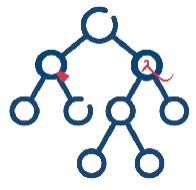
\includegraphics[height=1.0cm]{msca_logo.png}}%
    \end{center}

    \vspace{0.6cm}

    % Main title with Q logos on sides (with clickable links)
    \begin{center}
        \begin{minipage}{0.1\textwidth}
            \centering
            \href{https://quantlet.com}{
\includegraphics[height=1.1cm]{ql_logo.png}}
        \end{minipage}%
        \begin{minipage}{0.78\textwidth}
            \centering
            {\LARGE\bfseries\usebeamercolor[fg]{title}\inserttitle}

            \vspace{0.3cm}

            {\usebeamerfont{subtitle}\usebeamercolor[fg]{title}\insertsubtitle}
        \end{minipage}%
        \begin{minipage}{0.1\textwidth}
            \centering
            \href{https://quantinar.com}{
\includegraphics[height=1.1cm]{qr_logo.png}}
        \end{minipage}
    \end{center}

    \vspace{0.6cm}

    % Authors (left aligned)
    \hspace{0.5cm}{\usebeamerfont{author}\insertauthor}

    \vspace{0.3cm}

    % Institute/Affiliations (left aligned)
    \hspace{0.5cm}\begin{minipage}[t]{0.9\textwidth}
        \raggedright\small\insertinstitute
    \end{minipage}
}

%=============================================================================
% THEOREM ENVIRONMENTS
%=============================================================================
\theoremstyle{definition}
\setbeamertemplate{theorems}[numbered]
\ifdefined\tsalang
\newtheorem{defn}{Definiție}
\newtheorem{thm}{Teoremă}
\newtheorem{prop}{Propoziție}
\newtheorem{rmk}{Observație}
\else
\newtheorem{defn}{Definition}
\newtheorem{thm}{Theorem}
\newtheorem{prop}{Proposition}
\newtheorem{rmk}{Remark}
\fi

%=============================================================================
% CENTRED MINIPAGE (no extra vertical space)
%=============================================================================
\newenvironment{cminipage}[1]{%
    \par\noindent\hfill\begin{minipage}{#1}\ignorespaces
}{%
    \end{minipage}\hfill\null\par
}

%=============================================================================
% CUSTOM COMMANDS
%=============================================================================
\newcommand{\E}{\mathbb{E}}
\newcommand{\Var}{\text{Var}}
\newcommand{\Cov}{\text{Cov}}
\newcommand{\Corr}{\text{Corr}}
\newcommand{\R}{\mathbb{R}}
\newcommand{\N}{\mathbb{N}}
\newcommand{\Z}{\mathbb{Z}}
\newcommand{\B}{\mathbf{B}}
\newcommand{\imark}{\textcolor{MainBlue}{\textbullet}}
\newcommand{\RMSE}{\text{RMSE}}
\newcommand{\MAE}{\text{MAE}}
\newcommand{\MAPE}{\text{MAPE}}

% Boldface vector/matrix commands (VAR, VECM, state space; also used by the older TSA decks)
\newcommand{\bY}{\mathbf{Y}}
\newcommand{\bX}{\mathbf{X}}
\newcommand{\bA}{\mathbf{A}}
\newcommand{\bB}{\mathbf{B}}
\newcommand{\bepsilon}{\boldsymbol{\varepsilon}}
\newcommand{\bSigma}{\boldsymbol{\Sigma}}
\newcommand{\bPhi}{\boldsymbol{\Phi}}
\newcommand{\bGamma}{\boldsymbol{\Gamma}}
\newcommand{\bPi}{\boldsymbol{\Pi}}
\newcommand{\bc}{\mathbf{c}}
\newcommand{\balpha}{\boldsymbol{\alpha}}
\newcommand{\bbeta}{\boldsymbol{\beta}}
\newcommand{\bvarepsilon}{\boldsymbol{\varepsilon}}

% Legacy seminar marks (older TSA seminar decks)
\newcommand{\correct}{\textcolor{Forest}{\checkmark}}
\newcommand{\incorrect}{\textcolor{Crimson}{\texttimes}}
 se definește
%   \newcommand{\coursename}{Time Series Analysis}      (EN)
%   \newcommand{\coursename}{Serii de timp}       (RO)  și  \def\tsalang{ro}
% Fișierele .tex se află în EN/Courses, EN/Seminars, RO/Cursuri, RO/Seminarii (două niveluri sub rădăcină).
% Deck-urile sînt generate de latex/build_chapterN.py / build_seminarN.py (vezi latex/tsa_build.py).

\documentclass[9pt, aspectratio=169, t]{beamer}
\providecommand{\coursename}{Time Series Analysis}

% Ensure content fits on slides
\setbeamersize{text margin left=8mm, text margin right=8mm}
% Smaller institute font (title page)
\setbeamerfont{institute}{size=\footnotesize}

%=============================================================================
% THEME AND STYLE CONFIGURATION
%=============================================================================
\usetheme{default}
% Using default theme for clean header/footer control

% Color Palette (matching Redispatch PDF)
\definecolor{MainBlue}{RGB}{26, 58, 110}
\definecolor{AccentBlue}{RGB}{26, 58, 110}
\definecolor{IDAred}{RGB}{205, 0, 0}
\definecolor{DarkGray}{RGB}{51, 51, 51}
\definecolor{MediumGray}{RGB}{128, 128, 128}
\definecolor{LightGray}{RGB}{248, 248, 248}
\definecolor{VeryLightGray}{RGB}{235, 235, 235}
\definecolor{KeynoteGray}{RGB}{218, 218, 218}
\definecolor{SectionGray}{RGB}{120, 120, 120}
\definecolor{FooterGray}{RGB}{100, 100, 100}
\definecolor{Crimson}{RGB}{220, 53, 69}
\definecolor{Forest}{RGB}{46, 125, 50}
\definecolor{Amber}{RGB}{181, 133, 63}
\definecolor{Orange}{RGB}{230, 126, 34}
\definecolor{Purple}{RGB}{142, 68, 173}

% Gradient background (exact Keynote 315° gradient: white to RGB 218,218,218)
\setbeamertemplate{background}{%
    \begin{tikzpicture}[remember picture, overlay]
        \shade[shading=axis, shading angle=315,
        top color=white, bottom color=KeynoteGray]
        (current page.south west) rectangle (current page.north east);
    \end{tikzpicture}%
}
% Fallback solid color for compatibility
\setbeamercolor{background canvas}{bg=}

\setbeamercolor{palette primary}{bg=MainBlue, fg=white}
\setbeamercolor{palette secondary}{bg=MainBlue!85, fg=white}
\setbeamercolor{palette tertiary}{bg=MainBlue!70, fg=white}
\setbeamercolor{structure}{fg=MainBlue}
\setbeamercolor{title}{fg=IDAred}
\setbeamercolor{frametitle}{fg=IDAred, bg=}
\setbeamercolor{block title}{bg=MainBlue, fg=white}
\setbeamercolor{block body}{bg=VeryLightGray, fg=DarkGray}
\setbeamercolor{block title alerted}{bg=Crimson, fg=white}
\setbeamercolor{block body alerted}{bg=Crimson!8, fg=DarkGray}
\setbeamercolor{block title example}{bg=Forest, fg=white}
\setbeamercolor{block body example}{bg=Forest!8, fg=DarkGray}
\setbeamercolor{item}{fg=MainBlue}

% Footer colors (override Madrid theme blue)
\setbeamercolor{author in head/foot}{fg=FooterGray, bg=}
\setbeamercolor{title in head/foot}{fg=FooterGray, bg=}
\setbeamercolor{date in head/foot}{fg=FooterGray, bg=}
\setbeamercolor{section in head/foot}{fg=FooterGray, bg=}
\setbeamercolor{subsection in head/foot}{fg=FooterGray, bg=}

% Bullet styles (apply everywhere including blocks)
\setbeamertemplate{itemize item}{\color{MainBlue}$\boxdot$}
\setbeamertemplate{itemize subitem}{\color{MainBlue}$\blacktriangleright$}
\setbeamertemplate{itemize subsubitem}{\color{MainBlue}\tiny$\bullet$}
\setbeamertemplate{itemize/enumerate body begin}{\normalsize}
\setbeamertemplate{itemize/enumerate subbody begin}{\normalsize}

% Item spacing - compact style
\setlength{\leftmargini}{10pt}       % Level 1: minimal indent
\setlength{\leftmarginii}{10pt}      % Level 2: minimal additional indent
% Compact list spacing (zero extra space before/after lists in blocks)
\makeatletter
\def\@listi{\leftmargin\leftmargini \topsep 0pt \parsep 0pt \itemsep 0pt}
\def\@listii{\leftmargin\leftmarginii \topsep 0pt \parsep 0pt \itemsep 0pt}
\makeatother

\setbeamertemplate{navigation symbols}{}

%=============================================================================
% CUSTOM HEADLINE
%=============================================================================
\setbeamertemplate{headline}{%
    \vskip10pt%
    \hbox to \paperwidth{%
        \hskip0.5cm%
        {\small\color{FooterGray}\renewcommand{\hyperlink}[2]{##2}\insertsectionhead}%
        \hfill%
        \textcolor{FooterGray}{\small\insertframenumber}%
        \hskip0.5cm%
    }%
    \vskip4pt%
    {\color{FooterGray}\hrule height 0.4pt}%
}

%=============================================================================
% CUSTOM FOOTER
%=============================================================================
\usepackage{fontawesome5}

\setbeamertemplate{footline}{%
    {\color{FooterGray}\hrule height 0.4pt}%
    \vskip4pt%
    \hbox to \paperwidth{%
        \hskip0.5cm%
        \textcolor{FooterGray}{\small\coursename}%
        \hfill%
        \raisebox{-0.1em}{%
            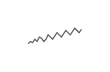
\begin{tikzpicture}[x=0.08em, y=0.08em, line width=0.4pt]
                \draw[FooterGray] (0,3) -- (1,4) -- (2,3.5) -- (3,5) -- (4,4) -- (5,6) -- (6,5.5) -- (7,4) -- (8,5) -- (9,7) -- (10,6) -- (11,5) -- (12,6.5) -- (13,8) -- (14,7) -- (15,6) -- (16,7.5) -- (17,9) -- (18,8) -- (19,7) -- (20,8.5) -- (21,10) -- (22,9) -- (23,8) -- (24,9.5);
            \end{tikzpicture}%
        }%
        \hskip0.5cm%
    }%
    \vskip6pt%
}

%=============================================================================
% PACKAGES
%=============================================================================
\usepackage[utf8]{inputenc}
\DeclareUnicodeCharacter{03B1}{\ensuremath{\alpha}}
\usepackage[T1]{fontenc}
\usepackage{amsmath, amssymb, amsthm}
\usepackage{mathtools}
\usepackage{bm}
\usepackage{tikz}
\usetikzlibrary{arrows.meta, positioning, shapes, calc, decorations.pathreplacing, shadings}
\usepackage{booktabs}
\usepackage{multirow}
\usepackage{array}
\usepackage{graphicx}
\usepackage{animate}
\usepackage{hyperref}
\usepackage{colortbl}
\usepackage{listings}
\lstset{language=Python, basicstyle=\ttfamily\scriptsize, keywordstyle=\color{MainBlue}\bfseries,
  commentstyle=\color{Forest}, stringstyle=\color{Crimson}, breaklines=true,
  frame=none, backgroundcolor=\color{VeryLightGray}, xleftmargin=2mm}
\hypersetup{colorlinks=true, linkcolor=MainBlue, urlcolor=MainBlue}
\graphicspath{{../../logos/}{../../charts/}{../../photos/}}
\usepackage{xcolor}
\hfuzz=2pt  % Suppress tiny overfull warnings (<2pt)
\vfuzz=2pt  % Suppress tiny vertical overfull warnings (<2pt)
% \mathrm in the sans-serif family of the slides (beamer resets \mathrm to the serif family at \begin{document};
% this hook runs after beamer's, so WN, Var, RMSE, ... in formulas match the surrounding text)
% Bold vectors and matrices in the same sans-serif family: \mathbf{A} in sans bold (beamer's own \mathbf came out in
% medium weight), and the bold upright Greek capitals of \boldsymbol / \bm (\bSigma, \bPhi, \boldsymbol{\Theta}) in
% cmss bold: bm.sty fixes its "boldoperators" font when it is loaded (serif cmbx), before beamer switches the
% operators to cmss, so it is reset here.
\AtBeginDocument{%
  \SetMathAlphabet{\mathrm}{normal}{\encodingdefault}{\sfdefault}{\mddefault}{n}%
  \SetMathAlphabet{\mathrm}{bold}{\encodingdefault}{\sfdefault}{bx}{n}%
  \SetMathAlphabet{\mathbf}{normal}{\encodingdefault}{\sfdefault}{bx}{n}%
  \SetMathAlphabet{\mathbf}{bold}{\encodingdefault}{\sfdefault}{bx}{n}%
  \SetSymbolFont{boldoperators}{normal}{OT1}{cmss}{bx}{n}%
  \SetSymbolFont{boldoperators}{bold}{OT1}{cmss}{bx}{n}}

%=============================================================================
% QUANTLET COMMANDS
%   \quantlet{<displayed name>}{<url>}       (generic, compatible with the older TSA decks)
%   \tsaquantlet{Ch_05}{TSA_ch5_garch}       -> https://github.com/danpele/Time-Series-Analysis/tree/main/Quantlets/Ch_05/TSA_ch5_garch
%   \qlurl{<folder>} is defined per chapter by the generator (Quantlets/Ch_NN/<folder>)
%=============================================================================
\newcommand{\tsarepo}{https://github.com/danpele/Time-Series-Analysis}
\newcommand{\tsaqlbase}{https://github.com/danpele/Time-Series-Analysis/tree/main/Quantlets}
\newcommand{\quantlet}[2]{%
    \hfill\href{#2}{%
        \raisebox{-0.15em}{
\includegraphics[height=0.7em]{ql_logo.png}}%
        \textcolor{MainBlue}{\tiny\ #1}%
    }%
}
\newcommand{\tsaquantlet}[2]{\quantlet{\detokenize{#2}}{\tsaqlbase/#1/#2}}

%=============================================================================
% NOTEBOOKS (Google Colab)
%   \colaburl{notebooks/EN/chapter5_seminar_notebook.ipynb} -> the Colab link of a file in the TSA repo
%   \nb: the chapter notebook (each seminar deck redefines it with \renewcommand)
%=============================================================================
\newcommand{\colaburl}[1]{https://colab.research.google.com/github/danpele/Time-Series-Analysis/blob/main/#1}
\newcommand{\nb}{https://colab.research.google.com/github/danpele/Time-Series-Analysis/tree/main/notebooks/EN}
\newcommand{\nbname}{notebooks/EN}

%=============================================================================
% SLIDE HELPERS (used by the generators; the same as in MFM)
%=============================================================================
% local font size for list bodies (the preamble forces \normalsize)
\newcommand{\itemsize}[1]{\setbeamertemplate{itemize/enumerate body begin}{#1}\setbeamertemplate{itemize/enumerate subbody begin}{#1}}
\newcommand{\intitle}[1]{{\hypersetup{urlcolor=white}#1}}   % white links inside coloured title bars
\newcommand{\imgcap}[1]{{\scriptsize #1}\\[0.5mm]}          % caption under a photo
\newcommand{\imgcredit}[2]{{\tiny\color{FooterGray}\href{#1}{#2}}}   % image credit: source URL, author/licence
\newcommand{\aiprompt}[1]{{\ttfamily\color{MainBlue}#1}}     % a prompt to an AI assistant

%=============================================================================
% SEMINARS: student version by default; the instructor wrapper *_solutions.tex sets \solutionstrue
%=============================================================================
\makeatletter\@ifundefined{ifsolutions}{\expandafter\newif\csname ifsolutions\endcsname}{}\makeatother
\newcommand{\solonly}[1]{\ifsolutions #1\fi}
\newcommand{\propsub}{\ifsolutions\else\framesubtitle{\ifdefined\tsalang Rezolvarea se discută la seminar\else Solution discussed in class\fi}\fi}

%=============================================================================
% APPENDIX AND CHAPTER LINKS (latex/appendix_links.py writes the calls; it also re-declares these
% macros before \begin{document}, so the decks compile with or without this preamble block)
%=============================================================================
\providecommand{\tsaapplink}[3]{\hypertarget{#2}{}\hyperlink{#1}{\beamergotobutton{#3}}}
\providecommand{\tsaappback}[2]{\begin{tikzpicture}[remember picture,overlay]\node[anchor=south east] at ([xshift=-3mm,yshift=7mm]current page.south east){\hyperlink{#1}{\beamerreturnbutton{#2}}};\end{tikzpicture}}
\providecommand{\tsachlink}[2]{\href{#1}{#2}}
\providecommand{\tsachlinkt}[2]{\href{#1}{\usebeamercolor[fg]{frametitle}#2}}

%=============================================================================
% QUANTINAR COMMAND: link către un curs Quantinar (subiecte avansate)
%=============================================================================
\newcommand{\quantinar}[2]{%
    \href{#2}{%
        \raisebox{-0.15em}{
\includegraphics[height=0.8em]{qr_logo.png}}%
        \textcolor{MainBlue}{\scriptsize\ #1}%
    }%
}

%=============================================================================
% CUSTOM TITLE PAGE
%=============================================================================
\defbeamertemplate*{title page}{hybrid}[1][]
{
    \vspace{0.2cm}
    % Logos row - top header (with clickable links)
    \begin{center}
        \href{https://www.ase.ro}{
\includegraphics[height=1.0cm]{ase_logo.png}}\hspace{0.3cm}%
        \href{https://theida.net}{
\includegraphics[height=1.0cm]{ida_logo.png}}\hspace{0.3cm}%
        \href{https://blockchain-research-center.com}{
\includegraphics[height=1.0cm]{brc_logo.png}}\hspace{0.3cm}%
        \href{https://www.ai4efin.ase.ro}{
\includegraphics[height=1.0cm]{ai4efin_logo.png}}\hspace{0.3cm}%
        \href{https://ipe.ro/new}{
\includegraphics[height=1.0cm]{acad_logo.png}}\hspace{0.3cm}%
        \href{https://www.digital-finance-msca.com}{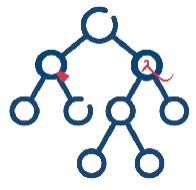
\includegraphics[height=1.0cm]{msca_logo.png}}%
    \end{center}

    \vspace{0.6cm}

    % Main title with Q logos on sides (with clickable links)
    \begin{center}
        \begin{minipage}{0.1\textwidth}
            \centering
            \href{https://quantlet.com}{
\includegraphics[height=1.1cm]{ql_logo.png}}
        \end{minipage}%
        \begin{minipage}{0.78\textwidth}
            \centering
            {\LARGE\bfseries\usebeamercolor[fg]{title}\inserttitle}

            \vspace{0.3cm}

            {\usebeamerfont{subtitle}\usebeamercolor[fg]{title}\insertsubtitle}
        \end{minipage}%
        \begin{minipage}{0.1\textwidth}
            \centering
            \href{https://quantinar.com}{
\includegraphics[height=1.1cm]{qr_logo.png}}
        \end{minipage}
    \end{center}

    \vspace{0.6cm}

    % Authors (left aligned)
    \hspace{0.5cm}{\usebeamerfont{author}\insertauthor}

    \vspace{0.3cm}

    % Institute/Affiliations (left aligned)
    \hspace{0.5cm}\begin{minipage}[t]{0.9\textwidth}
        \raggedright\small\insertinstitute
    \end{minipage}
}

%=============================================================================
% THEOREM ENVIRONMENTS
%=============================================================================
\theoremstyle{definition}
\setbeamertemplate{theorems}[numbered]
\ifdefined\tsalang
\newtheorem{defn}{Definiție}
\newtheorem{thm}{Teoremă}
\newtheorem{prop}{Propoziție}
\newtheorem{rmk}{Observație}
\else
\newtheorem{defn}{Definition}
\newtheorem{thm}{Theorem}
\newtheorem{prop}{Proposition}
\newtheorem{rmk}{Remark}
\fi

%=============================================================================
% CENTRED MINIPAGE (no extra vertical space)
%=============================================================================
\newenvironment{cminipage}[1]{%
    \par\noindent\hfill\begin{minipage}{#1}\ignorespaces
}{%
    \end{minipage}\hfill\null\par
}

%=============================================================================
% CUSTOM COMMANDS
%=============================================================================
\newcommand{\E}{\mathbb{E}}
\newcommand{\Var}{\text{Var}}
\newcommand{\Cov}{\text{Cov}}
\newcommand{\Corr}{\text{Corr}}
\newcommand{\R}{\mathbb{R}}
\newcommand{\N}{\mathbb{N}}
\newcommand{\Z}{\mathbb{Z}}
\newcommand{\B}{\mathbf{B}}
\newcommand{\imark}{\textcolor{MainBlue}{\textbullet}}
\newcommand{\RMSE}{\text{RMSE}}
\newcommand{\MAE}{\text{MAE}}
\newcommand{\MAPE}{\text{MAPE}}

% Boldface vector/matrix commands (VAR, VECM, state space; also used by the older TSA decks)
\newcommand{\bY}{\mathbf{Y}}
\newcommand{\bX}{\mathbf{X}}
\newcommand{\bA}{\mathbf{A}}
\newcommand{\bB}{\mathbf{B}}
\newcommand{\bepsilon}{\boldsymbol{\varepsilon}}
\newcommand{\bSigma}{\boldsymbol{\Sigma}}
\newcommand{\bPhi}{\boldsymbol{\Phi}}
\newcommand{\bGamma}{\boldsymbol{\Gamma}}
\newcommand{\bPi}{\boldsymbol{\Pi}}
\newcommand{\bc}{\mathbf{c}}
\newcommand{\balpha}{\boldsymbol{\alpha}}
\newcommand{\bbeta}{\boldsymbol{\beta}}
\newcommand{\bvarepsilon}{\boldsymbol{\varepsilon}}

% Legacy seminar marks (older TSA seminar decks)
\newcommand{\correct}{\textcolor{Forest}{\checkmark}}
\newcommand{\incorrect}{\textcolor{Crimson}{\texttimes}}


\newcommand{\qlurl}[1]{https://github.com/danpele/Time-Series-Analysis/tree/main/Quantlets/Ch_13/#1}

% Clickable citations (DOIs verified via Crossref)
\newcommand{\refHP}{\href{https://doi.org/10.1007/978-3-031-13584-2}{Huang and Petukhina (2022)}}
\newcommand{\refJLS}{\href{https://doi.org/10.1142/S0219024900000115}{Johansen, Ledoit and Sornette (2000)}}
\newcommand{\refSJB}{\href{https://doi.org/10.1051/jp1:1996135}{Sornette, Johansen and Bouchaud (1996)}}
\newcommand{\refSornette}{\href{https://doi.org/10.23943/princeton/9780691175959.001.0001}{Sornette (2017)}}
\newcommand{\refFS}{\href{https://doi.org/10.1016/j.physa.2013.04.012}{Filimonov and Sornette (2013)}}
\newcommand{\refSZ}{\href{https://doi.org/10.1016/j.physa.2020.124892}{Shu and Zhu (2020)}}
\newcommand{\refShanghai}{\href{https://doi.org/10.21314/JOIS.2015.063}{Sornette et al.\ (2015)}}
\newcommand{\refJiang}{\href{https://doi.org/10.1016/j.jebo.2010.02.007}{Jiang et al.\ (2010)}}
\newcommand{\refGerlach}{\href{https://doi.org/10.1098/rsos.180643}{Gerlach, Demos and Sornette (2019)}}
\newcommand{\refFeig}{\href{https://doi.org/10.1088/1469-7688/1/3/306}{Feigenbaum (2001)}}
\newcommand{\refBJ}{\href{https://doi.org/10.1016/j.irfa.2013.05.005}{Brée and Joseph (2013)}}
\newcommand{\refLomb}{\href{https://doi.org/10.1007/BF00648343}{Lomb (1976)}}
\newcommand{\refBW}{\href{https://doi.org/10.3386/w0945}{Blanchard and Watson (1982)}}
\newcommand{\refPWY}{\href{https://doi.org/10.1111/j.1468-2354.2010.00625.x}{Phillips, Wu and Yu (2011)}}
\newcommand{\refPSYa}{\href{https://doi.org/10.1111/iere.12132}{Phillips, Shi and Yu (2015a)}}
\newcommand{\refPSYb}{\href{https://doi.org/10.1111/iere.12131}{Phillips, Shi and Yu (2015b)}}
\newcommand{\refPS}{\href{https://doi.org/10.1016/bs.host.2018.12.002}{Phillips and Shi (2020)}}
\newcommand{\refDF}{\href{https://doi.org/10.1080/01621459.1979.10482531}{Dickey and Fuller (1979)}}
\newcommand{\refGarber}{\href{https://doi.org/10.1257/jep.4.2.35}{Garber (1990)}}
\newcommand{\refKA}{\href{https://doi.org/10.1057/9780230628045}{Kindleberger and Aliber (2005)}}
\newcommand{\refShiller}{\href{https://doi.org/10.1515/9781400865536}{Shiller (2015)}}
\newcommand{\refFama}{\href{https://doi.org/10.1257/aer.104.6.1467}{Fama (2014)}}
\newcommand{\refGSY}{\href{https://doi.org/10.1016/j.jfineco.2018.09.002}{Greenwood, Shleifer and You (2019)}}
\newcommand{\refPeleCrash}{\href{https://doi.org/10.1016/j.sbspro.2012.09.1030}{Pele and Mazurencu-Marinescu (2012)}}

\title[Time Series Analysis]{Time Series Analysis}
\subtitle{Chapter 13: Speculative bubbles: LPPL models}
\author[D.T. Pele]{Daniel Traian PELE}
\institute{Bucharest University of Economic Studies\\
IDA Institute Digital Assets\\
Blockchain Research Center\\
AI4EFin Artificial Intelligence for Energy Finance\\
Romanian Academy, Institute for Economic Forecasting\\
MSCA Digital Finance}
\date{}

%=============================================================================
\providecommand{\tsaapplink}[3]{\hypertarget{#2}{}\hyperlink{#1}{\beamergotobutton{#3}}}  % APPLINKS-MACROS
\providecommand{\tsaappback}[2]{\begin{tikzpicture}[remember picture,overlay]\node[anchor=south east] at ([xshift=-3mm,yshift=7mm]current page.south east){\hyperlink{#1}{\beamerreturnbutton{#2}}};\end{tikzpicture}}  % APPLINKS-MACROS
\providecommand{\tsachlink}[2]{\href{#1}{#2}}  % APPLINKS-MACROS
\providecommand{\tsachlinkt}[2]{\href{#1}{\usebeamercolor[fg]{frametitle}#2}}  % APPLINKS-MACROS
\begin{document}
%=============================================================================

{
\setbeamertemplate{headline}{}
\setbeamertemplate{footline}{}
\begin{frame}[noframenumbering]
    \titlepage
\end{frame}
}
% BEGIN-ACRONYMS (generat de latex/acronyms.py; nu editati manual)
\begin{frame}{Acronyms used in this material}
\setbeamertemplate{itemize/enumerate body begin}{\footnotesize}
\begin{columns}[T]
\begin{column}{0.49\textwidth}
\begin{itemize}\setlength{\itemsep}{0pt}
    \item \textbf{ADF}: Augmented Dickey–Fuller (test)
    \item \textbf{AI}: Artificial Intelligence
    \item \textbf{AR}: AutoRegressive (model)
    \item \textbf{BET}: Bucharest Exchange Trading (index)
    \item \textbf{BET-TR}: BET Total Return (index)
    \item \textbf{BSADF}: Backward Supremum Augmented Dickey–Fuller (statistic)
    \item \textbf{EODHD}: EOD Historical Data (market-data provider)
    \item \textbf{GARCH}: Generalised AutoRegressive Conditional Heteroskedasticity
\end{itemize}
\end{column}
\begin{column}{0.49\textwidth}
\begin{itemize}\setlength{\itemsep}{0pt}
    \item \textbf{GSADF}: Generalised Supremum Augmented Dickey–Fuller (test)
    \item \textbf{JLS}: Johansen–Ledoit–Sornette (model)
    \item \textbf{LPPL}: Log-Periodic Power Law
    \item \textbf{LPPLS}: Log-Periodic Power Law Singularity (model)
    \item \textbf{OLS}: Ordinary Least Squares
    \item \textbf{SADF}: Supremum Augmented Dickey–Fuller (test)
    \item \textbf{SE}: Standard Error
    \item \textbf{SSR}: Sum of Squared Residuals
\end{itemize}
\end{column}
\end{columns}
\end{frame}
% END-ACRONYMS

%=============================================================================
\section{Motivation}
%=============================================================================

\begin{frame}{The question of the chapter}
\itemsize{\small}
\begin{itemize}
    \item \textbf{Question}: can a speculative bubble be recognised in a price series before it bursts?
    \begin{itemize}
        \item a \textbf{speculative bubble}: a price that rises far above the value justified by the expected cash flows of the asset, sustained by the expectation of selling it later at a higher price
        \item a \textbf{crash}: a large fall of the price in a short time (here: at least 20\% from the peak)
    \end{itemize}
    \item \textbf{Route} of the chapter
    \begin{itemize}
        \item bubbles in history and the statistical signatures of a bubble
        \item rational bubbles and explosive roots: the right-tailed unit-root tests of Phillips, Shi and Yu (link with \tsachlink{https://danpele.github.io/Time-Series-Analysis/EN/Courses/chapter3_unit_roots_arima_models.pdf}{Chapter 3})
        \item the LPPL model of Johansen, Ledoit and Sornette: super-exponential growth, log-periodic oscillations, the critical time
        \item estimation, confidence from many windows and an honest evaluation of crash prediction
    \end{itemize}
\end{itemize}
\end{frame}

\begin{frame}{Self-study guide}
\itemsize{\small}
\begin{itemize}
    \item This chapter is for \textbf{self-study}
    \begin{itemize}
        \item there is no seminar
        \item each section ends with a recap
        \item read a section, then redo its worked example on paper before you look at the solution
        \item after each chart, read the interpretation slide and compare it with your own reading of the chart
    \end{itemize}
    \item Run the lecture notebook: every chart and number of the slides is produced there
    \begin{itemize}
        \item change one setting (the window, the filter, the threshold) and see how the conclusion changes
    \end{itemize}
    \item Check yourself with the self-assessment at the end and with the quiz of \tsachlink{https://danpele.github.io/Time-Series-Analysis/EN/Courses/chapter13_bubbles_lppl.pdf}{Chapter 13} on the course site
    \item Prerequisites: log returns and log prices (\tsachlink{https://danpele.github.io/Time-Series-Analysis/EN/Courses/chapter1_stochastic_processes_stationarity.pdf}{Chapter 1}), the Dickey--Fuller test (\tsachlink{https://danpele.github.io/Time-Series-Analysis/EN/Courses/chapter3_unit_roots_arima_models.pdf}{Chapter 3}), OLS regression
\end{itemize}
\end{frame}

\begin{frame}{Learning outcomes}
\itemsize{\small}
\begin{itemize}
    \item Describe a bubble by its fundamental value and by its statistical signatures
    \item Explain why a rational bubble must grow at an explosive rate and test for explosive roots with SADF and GSADF
    \item Write the LPPL equation and interpret each of its seven parameters
    \item Estimate LPPL with the two-step method of Filimonov and Sornette and check the filter conditions
    \item Build a confidence indicator from many windows and evaluate its alarms honestly, with false alarms and base rates
\end{itemize}
\end{frame}

\begin{frame}{Reading and tools}
\itemsize{\small}
\begin{itemize}
    \item Textbook background: \refHP\ (unit roots and nonlinear least squares, the tools of this chapter)
    \begin{itemize}
        \item the LPPL model: \refJLS; \refSornette; calibration: \refFS
        \item explosive roots: \refPWY; \refPSYa; survey: \refPS
        \item history of bubbles: \refKA; \refShiller; \refGarber
    \end{itemize}
    \item Python Quantlets of this chapter: \href{https://github.com/danpele/Time-Series-Analysis/tree/main/Quantlets/Ch_13}{Quantlets/Ch\_13}
    \begin{itemize}
        \item the SADF/GSADF statistics and the LPPL calibration are written out in the code (no special package)
    \end{itemize}
    \item Lecture notebook: \href{\colaburl{notebooks/EN/chapter13_lecture_notebook.ipynb}}{open in Google Colab}
    \item Data: daily closes of the S\&P 500, Nasdaq 100, BET, Shanghai Composite and Bitcoin (EODHD)
\end{itemize}
\end{frame}


%=============================================================================
\section{Bubbles in history}
%=============================================================================

\begin{frame}{Four centuries of manias}
\itemsize{\footnotesize}
\begin{columns}[T]
\begin{column}{0.38\textwidth}
\centering
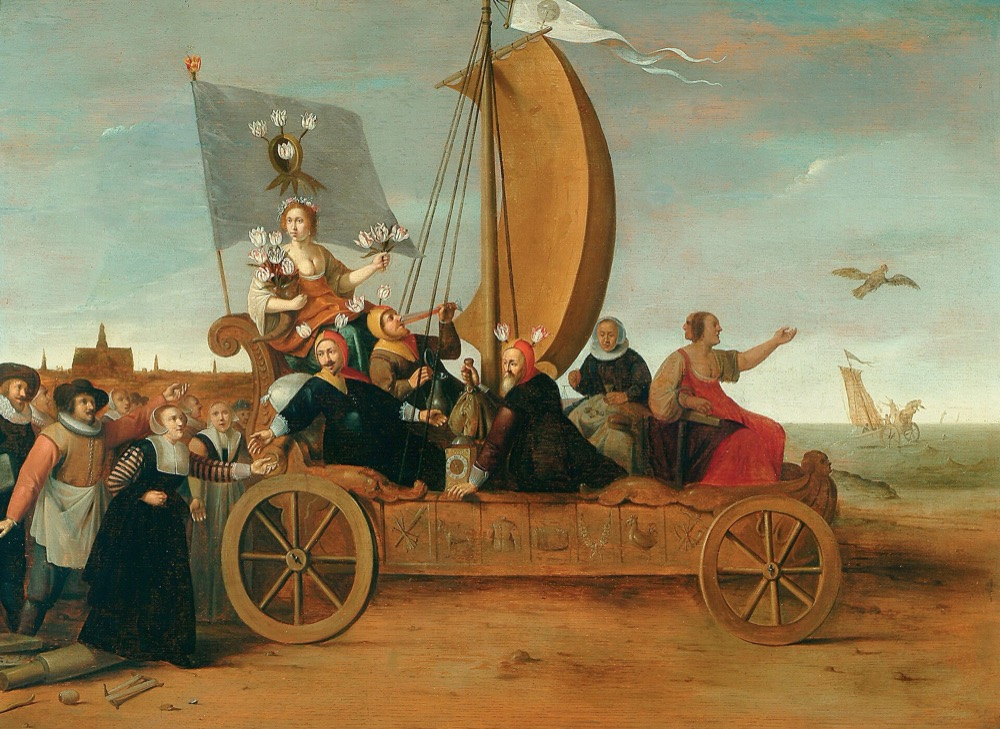
\includegraphics[height=0.36\textheight]{ch13_tulip_mania_1637.jpg}\\[1mm]
\imgcap{Flora's wagon of fools, c.~1637}
\imgcredit{https://commons.wikimedia.org/wiki/File:Flora's_Wagon_of_Fools_(Flora's_Mallewagen)_tulipomania,_Hendrik_Gerritsz_Pot_c1637.jpg}{Painting: Hendrik Gerritsz Pot (c.~1637); public domain; Wikimedia Commons}
\end{column}
\begin{column}{0.6\textwidth}
\begin{itemize}
    \item \textbf{Tulip mania}, Netherlands, 1636--1637
    \begin{itemize}
        \item contracts on rare bulbs traded at extreme prices, then collapsed in February 1637
        \item \refGarber: part of the story is a myth; rare bulbs were expensive for good reasons, common bulbs show the mania
    \end{itemize}
    \item \textbf{South Sea} (1720), \textbf{Wall Street} (1929), \textbf{Japan} (1989), \textbf{dot-com} (2000), \textbf{housing} (2007), \textbf{crypto} (2017, 2021)
    \item The common pattern \refKA: a new story, easy credit, rising prices that attract new buyers, then panic
\end{itemize}
\end{column}
\end{columns}
\end{frame}

\begin{frame}{1929 and 1987}
\itemsize{\footnotesize}
\begin{columns}[T]
\begin{column}{0.38\textwidth}
\centering
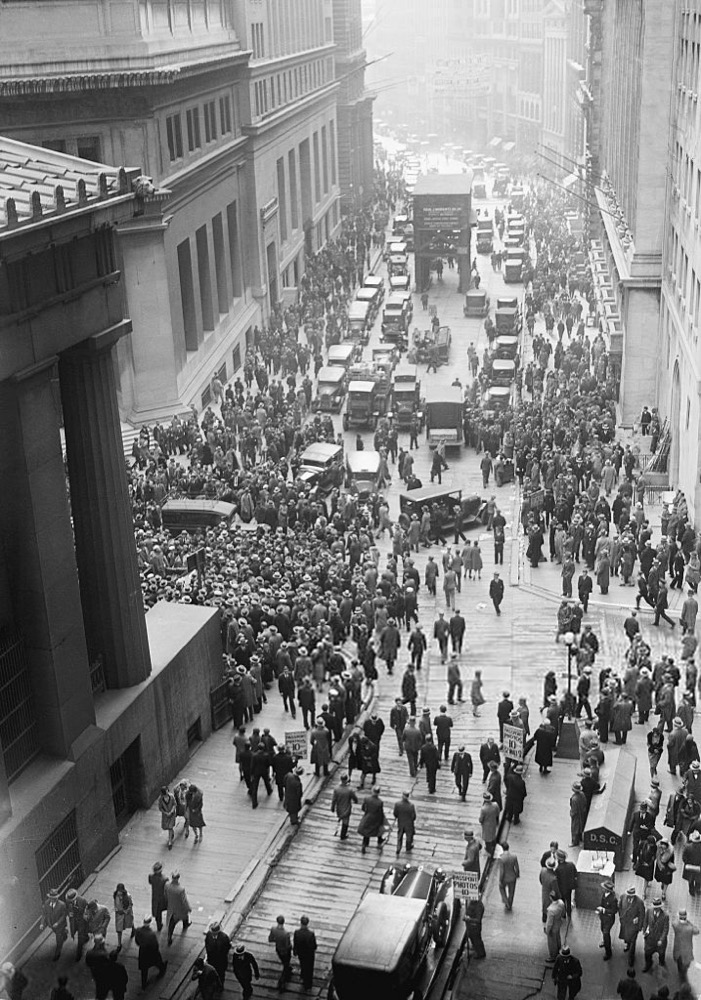
\includegraphics[height=0.25\textheight]{ch13_nyse_crowd_1929.jpg}\\[1mm]
\imgcap{Crowd outside the New York Stock Exchange, 29 October 1929}
\imgcredit{https://commons.wikimedia.org/wiki/File:Crowd_outside_nyse.jpg}{Photo: US government (1929); public domain; Wikimedia Commons}
\par\vspace{2mm}
\centering
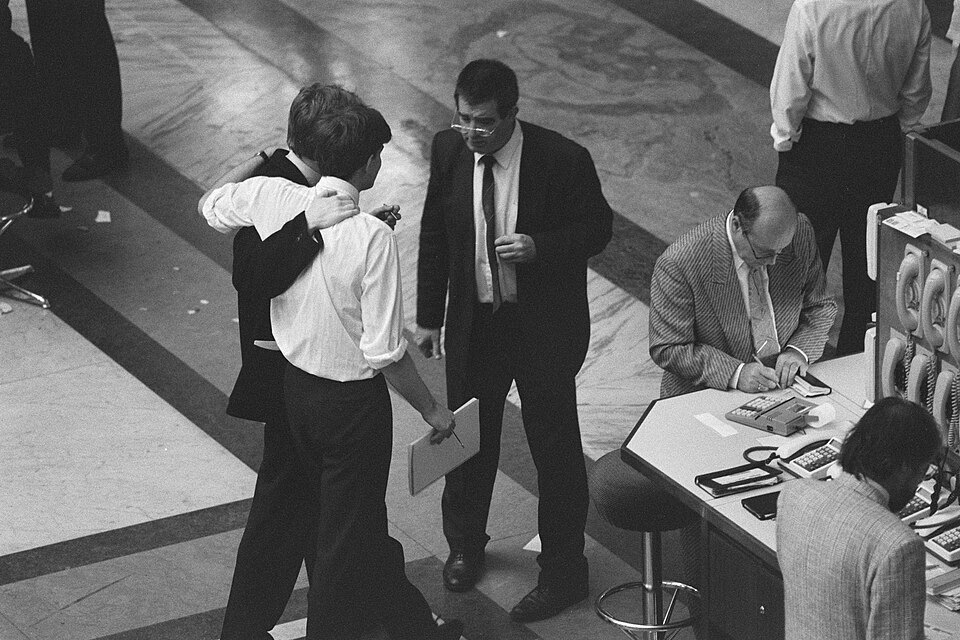
\includegraphics[height=0.16\textheight]{ch13_amsterdam_crash_1987.jpg}\\[1mm]
\imgcap{Amsterdam Stock Exchange, 21 October 1987}
\imgcredit{https://commons.wikimedia.org/wiki/File:Effectenbeurs_Amsterdam_na_koersval,_Bestanddeelnr_934-1094.jpg}{Photo: Bart Molendijk / Anefo, Nationaal Archief (1987); CC0; Wikimedia Commons}
\end{column}
\begin{column}{0.6\textwidth}
\begin{itemize}
    \item \textbf{October 1929}
    \begin{itemize}
        \item the end of the boom of the 1920s and the start of the Great Depression
    \end{itemize}
    \item \textbf{19 October 1987} (Black Monday)
    \begin{itemize}
        \item the largest one-day fall of the Dow Jones index, without any major news that day
        \item \refSJB\ found accelerating, log-periodic oscillations in the years before 1987; this observation started the LPPL literature
        \item the daily data of this course start in 1990: we study 1987 through the literature and later bubbles with our own data
    \end{itemize}
    \item A crash without news suggests an \textbf{endogenous} cause: the market itself became fragile
\end{itemize}
\end{column}
\end{columns}
\end{frame}

\begin{frame}{Fundamental value and bubble}
\itemsize{\footnotesize}
\begin{itemize}
    \item \textbf{Fundamental value} $F_t$
    \begin{itemize}
        \item the present value of the expected future cash flows (dividends $D$), discounted at the rate $r$
        \item $F_t = \sum_{k=1}^{\infty} \dfrac{E_t[D_{t+k}]}{(1+r)^k}$
        \item $D_{t+k}$: the dividend paid $k$ periods from now; $E_t[\cdot]$: the expectation given the information available at $t$; $r$: the discount rate per period
    \end{itemize}
    \item \textbf{Bubble component}
    \begin{itemize}
        \item $B_t = P_t - F_t$, the part of the price $P_t$ not explained by fundamentals
        \item $F_t$ is not observed: we can only test the \textbf{implications} of a bubble in the price path
    \end{itemize}
    \item Two views
    \begin{itemize}
        \item efficient markets: prices reflect information; ``bubbles'' are visible only with hindsight \refFama
        \item behavioural finance: herding and extrapolation push prices away from value \refShiller; large run-ups do raise the probability of a crash \refGSY
    \end{itemize}
\end{itemize}
\end{frame}

\begin{frame}{Six run-ups and crashes in the course data}
\itemsize{\footnotesize}
\begin{center}
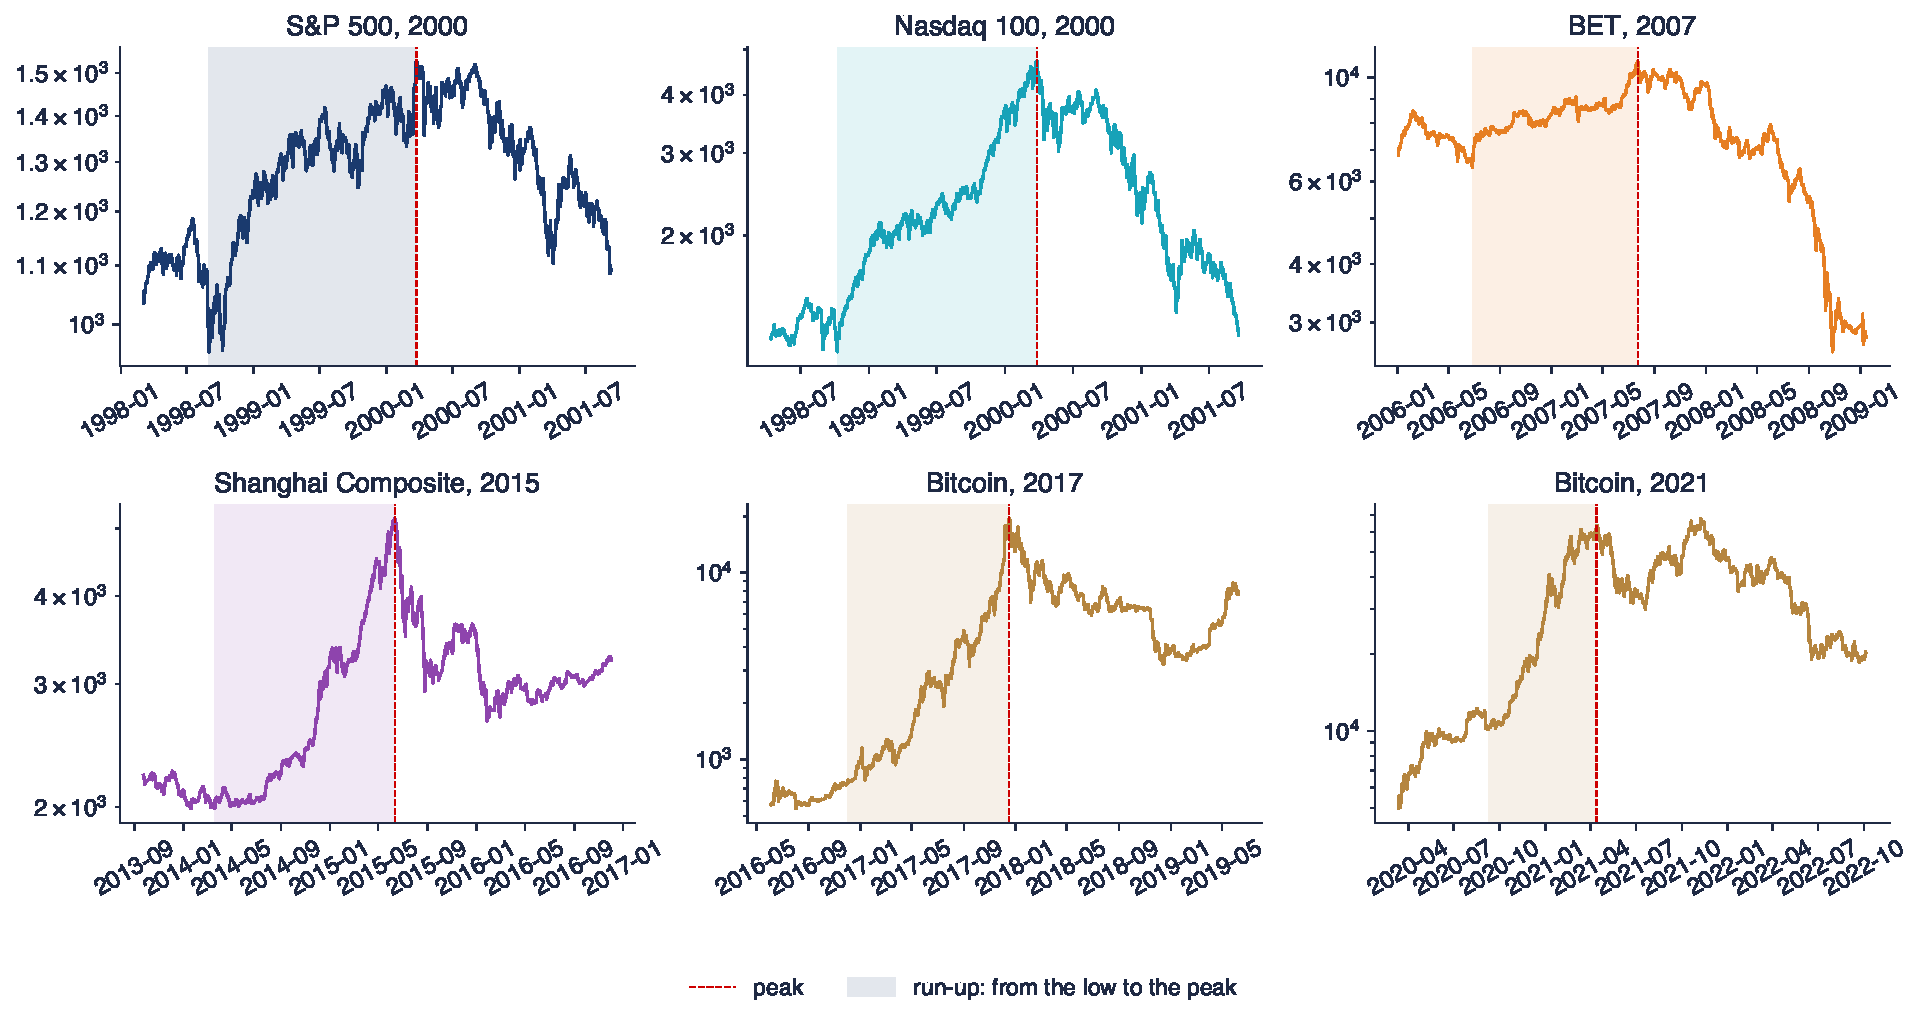
\includegraphics[width=0.97\textwidth,height=0.66\textheight,keepaspectratio]{tsa_ch13_episodes.pdf}
\end{center}
\vspace{-0.25cm}
\begin{itemize}
    \item Daily closes, log scale, from six months before the low of the run-up to eighteen months after the peak; shaded: the run-up from the low to the peak
\end{itemize}
\quantlet{TSA\_ch13\_episodes}{\qlurl{TSA_ch13_episodes}}
\end{frame}

\begin{frame}{Interpreting the six episodes}
\itemsize{\footnotesize}
\setlength{\tabcolsep}{4pt}\begin{center}
\scriptsize
\begin{tabular}{lllrrr}
\toprule
\textbf{Episode} & \textbf{Low} & \textbf{Peak} & \textbf{Rise} & \textbf{Growth p.a.} & \textbf{Fall in 1 year} \\
\midrule
S\&P 500, 2000 & 31 August 1998 & 24 March 2000 & 60\% & 30\% & 27\% \\
Nasdaq 100, 2000 & 8 October 1998 & 27 March 2000 & 317\% & 97\% & 66\% \\
BET, 2007 & 27 June 2006 & 24 July 2007 & 68\% & 48\% & 50\% \\
Shanghai Composite, 2015 & 20 March 2014 & 12 June 2015 & 159\% & 77\% & 49\% \\
Bitcoin, 2017 & 1 December 2016 & 16 December 2017 & 2476\% & 312\% & 83\% \\
Bitcoin, 2021 & 8 September 2020 & 13 April 2021 & 527\% & 309\% & 53\% \\
\bottomrule
\end{tabular}
\end{center}
\begin{itemize}
    \item Growth p.a.: $\ln(P_{\text{peak}}/P_{\text{low}})$ divided by the length of the run-up in years; fall: the lowest close in the year after the peak, relative to the peak
    \item Bitcoin multiplied its price 26 times in about a year; the S\&P 500 rose much less: not every peak is a bubble of the same strength
\end{itemize}
\end{frame}

\begin{frame}{Recap: Bubbles in history}
\itemsize{\small}
\begin{itemize}
    \item A bubble is a price above the fundamental value $F_t$; $F_t$ is not observed
    \item Six episodes in our data: run-ups of 60\% to 2476\%, followed by falls of 27\% to 83\% within a year
    \item Signatures: explosive and super-exponential growth, accelerating oscillations, then an end
\end{itemize}
\end{frame}


%=============================================================================
\section{Rational bubbles and explosive roots}
%=============================================================================

\begin{frame}{Why a rational bubble must explode}
\itemsize{\footnotesize}
\begin{itemize}
    \item No-arbitrage pricing: $P_t = \dfrac{E_t[P_{t+1} + D_{t+1}]}{1+r}$; the fundamental value $F_t$ is one solution
    \begin{itemize}
        \item in words: today's price is the discounted expected value of tomorrow's price plus tomorrow's dividend
        \item every $P_t = F_t + B_t$ with $E_t[B_{t+1}] = (1+r)\,B_t$ is also a solution
    \end{itemize}
    \item The bubble must grow, in expectation, at the rate $r$: $E_t[B_{t+k}] = (1+r)^k B_t$
    \begin{itemize}
        \item an investor holds an asset above its value only if the overvaluation is expected to grow
        \item $1+r > 1$: the bubble component is an \textbf{explosive} process
    \end{itemize}
    \item Consequence: if dividends are $I(1)$ (\tsachlink{https://danpele.github.io/Time-Series-Analysis/EN/Courses/chapter3_unit_roots_arima_models.pdf}{Chapter 3}), the price is $I(1)$ without a bubble and explosive with one
\end{itemize}
\end{frame}

\begin{frame}{Worked example: a bubble that can burst}
\itemsize{\small}
\begin{itemize}
    \item \refBW: each period the bubble survives with probability $\pi$ and then grows to $\frac{1+r}{\pi}B_t$; otherwise it bursts ($B_{t+1} \approx 0$)
    \begin{itemize}
        \item check: $E_t[B_{t+1}] = \pi \cdot \frac{1+r}{\pi} B_t + (1-\pi) \cdot 0 = (1+r)B_t$
    \end{itemize}
    \item With $r = 2\%$ and $\pi = 0.98$ per period:
    \begin{itemize}
        \item while it survives the bubble grows by $1.02/0.98 - 1 = 4.08\%$ per period, more than $r$: the extra growth pays for the risk of a burst
        \item expected lifetime $1/(1-\pi) = 50$ periods; it survives more than 34 periods with probability $1/2$ ($0.98^{k} = 0.5$)
    \end{itemize}
    \item The longer the bubble lasts, the faster it must grow and the larger the fall when it bursts
\end{itemize}
\end{frame}

\begin{frame}{A simulated rational bubble and three AR(1) roots}
\itemsize{\footnotesize}
\begin{center}
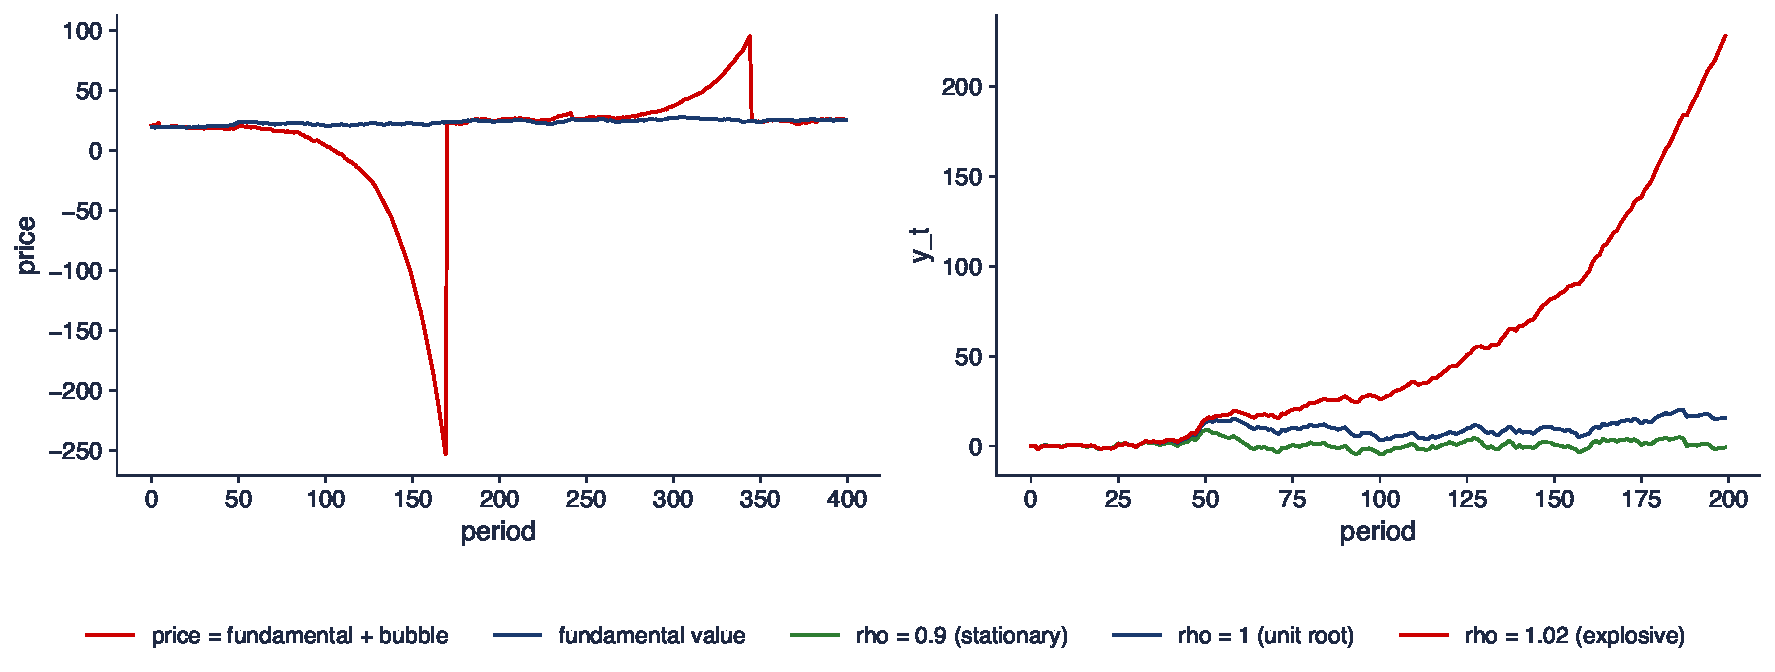
\includegraphics[width=0.97\textwidth,height=0.6\textheight,keepaspectratio]{tsa_ch13_rational.pdf}
\end{center}
\vspace{-0.25cm}
\begin{itemize}
    \item Left: fundamental value (random walk) plus a Blanchard--Watson bubble ($r = 2\%$, $\pi = 0.98$), 400 periods; right: $y_t = \rho y_{t-1} + \varepsilon_t$ with the same shocks and $\rho = 0.9$, $1$, $1.02$
\end{itemize}
\quantlet{TSA\_ch13\_rational\_bubble}{\qlurl{TSA_ch13_rational_bubble}}
\end{frame}

\begin{frame}{Interpreting the simulation}
\itemsize{\small}
\begin{itemize}
    \item The bubble grows, bursts, restarts: in this path it reaches 71 and bursts 2 times after a large size
    \begin{itemize}
        \item the price inherits the explosive episodes; between them it follows the fundamental value
    \end{itemize}
    \item AR(1) roots (\tsachlink{https://danpele.github.io/Time-Series-Analysis/EN/Courses/chapter3_unit_roots_arima_models.pdf}{Chapter 3}): $\rho = 0.9$ reverts to the mean, $\rho = 1$ wanders (unit root), $\rho = 1.02$ explodes
    \begin{itemize}
        \item with $\rho = 1.02$ a shock doubles in about 35 periods and is multiplied by 7.24 after 100
    \end{itemize}
    \item Idea of the tests: an explosive root ($\rho > 1$) in the log price during a run-up is the statistical trace of a rational bubble
\end{itemize}
\end{frame}

\begin{frame}{Right-tailed unit-root tests}
\itemsize{\footnotesize}
\begin{itemize}
    \item The regression of \tsachlink{https://danpele.github.io/Time-Series-Analysis/EN/Courses/chapter3_unit_roots_arima_models.pdf}{Chapter 3} on a window of the log price $y_t = \ln P_t$: $\Delta y_t = a + \delta\, y_{t-1} + \varepsilon_t$, with $\delta = \rho - 1$
    \begin{itemize}
        \item \tsachlink{https://danpele.github.io/Time-Series-Analysis/EN/Courses/chapter3_unit_roots_arima_models.pdf}{Chapter 3} (\refDF): $H_0$: $\delta = 0$ against $H_1$: $\delta < 0$ (stationary), the \textbf{left} tail
        \item bubbles: $H_0$: $\delta = 0$ (unit root) against $H_1$: $\delta > 0$ (explosive), the \textbf{right} tail: reject for large $t$-statistics
    \end{itemize}
    \item Problem: a bubble occupies only a part of the sample, and the crash after it looks like mean reversion
    \begin{itemize}
        \item one ADF on the whole sample has almost no power: we must compute the test on many \textbf{windows}
    \end{itemize}
    \item Notation
    \begin{itemize}
        \item $\Delta y_t = y_t - y_{t-1}$; $a$: the intercept; $\varepsilon_t$: the error; $\rho$: the AR(1) coefficient of $y_t$
        \item $r_1, r_2 \in [0,1]$: fractions of the sample; $\mathrm{ADF}_{r_1}^{r_2}$: the $t$-statistic of $\hat\delta$ on the window from $r_1T$ to $r_2T$; $r_0$: the smallest window
    \end{itemize}
\end{itemize}
\end{frame}

\begin{frame}{SADF, GSADF and BSADF (1/2)}
\itemsize{\small}
\begin{itemize}
    \item $\sup$: the largest value of the ADF statistic over all the windows considered
    \begin{itemize}
        \item a single large value, in any window, is enough to signal an explosive episode
    \end{itemize}
    \item \textbf{SADF} \refPWY
    \begin{itemize}
        \item start fixed at 0, the end $r_2$ moves forward
        \item $\mathrm{SADF} = \sup_{r_2 \in [r_0, 1]} \mathrm{ADF}_{0}^{r_2}$
        \item good for one bubble; after a first crash it loses power
    \end{itemize}
    \item \textbf{GSADF} \refPSYa
    \begin{itemize}
        \item both the start $r_1$ and the end $r_2$ move
        \item $\mathrm{GSADF} = \sup_{r_2 \in [r_0,1]}\ \sup_{r_1 \in [0, r_2 - r_0]} \mathrm{ADF}_{r_1}^{r_2}$
        \item detects several bubbles in one sample; smallest window $r_0 = 0.01 + 1.8/\sqrt{T}$
    \end{itemize}
\end{itemize}
\end{frame}

\begin{frame}{SADF, GSADF and BSADF (2/2)}
\itemsize{\small}
\begin{itemize}
    \item \textbf{BSADF} (date-stamping)
    \begin{itemize}
        \item one statistic for each date $r_2$, using only data up to $r_2$
        \item $\mathrm{BSADF}(r_2) = \sup_{r_1} \mathrm{ADF}_{r_1}^{r_2}$: the largest statistic over all starts $r_1$ of windows ending at $r_2$
        \item an episode starts when BSADF crosses its critical value and lasts at least $\log T$ observations \refPSYb{} ($\log$: the natural logarithm)
    \end{itemize}
    \item The distributions are not standard: critical values by Monte Carlo
    \begin{itemize}
        \item simulated under a random walk with a weak drift, $y_t = T^{-1} + y_{t-1} + \varepsilon_t$
        \item the drift $T^{-1}$ is very small: a unit root, not an explosive root, under $H_0$
    \end{itemize}
    \item Reading: an ADF, SADF or GSADF statistic above its 95\% critical value rejects the unit root in favour of an explosive root
\end{itemize}
\end{frame}

\begin{frame}{Worked example: one window of the Nasdaq 100}
\itemsize{\small}
\begin{itemize}
    \item Weekly log closes of the Nasdaq 100, $T = 782$ weeks; $r_0 = 0.074$, i.e.\ a smallest window of 58 weeks
    \begin{itemize}
        \item end of the window: 24 March 2000, the week of the peak; among all start points the largest statistic comes from the start 17 January 1992
    \end{itemize}
    \item OLS on this window ($n = 427$ weekly changes): $\widehat{\Delta y_t} = -0.0336 + 0.0060\, y_{t-1}$
    \begin{itemize}
        \item $t = \hat\delta / \mathrm{SE}(\hat\delta) = 0.0060 / 0.0021 = 2.91$
        \item so BSADF at the peak is 2.91, above its 95\% critical value of 0.54
    \end{itemize}
    \item Reading: $\hat\delta > 0$ means $\hat\rho = 1 + \hat\delta > 1$: the higher the price, the larger the next weekly rise, the mark of an explosive phase
\end{itemize}
\end{frame}

\begin{frame}{Explosive episodes of the Nasdaq 100, 1990--2004}
\itemsize{\footnotesize}
\begin{center}
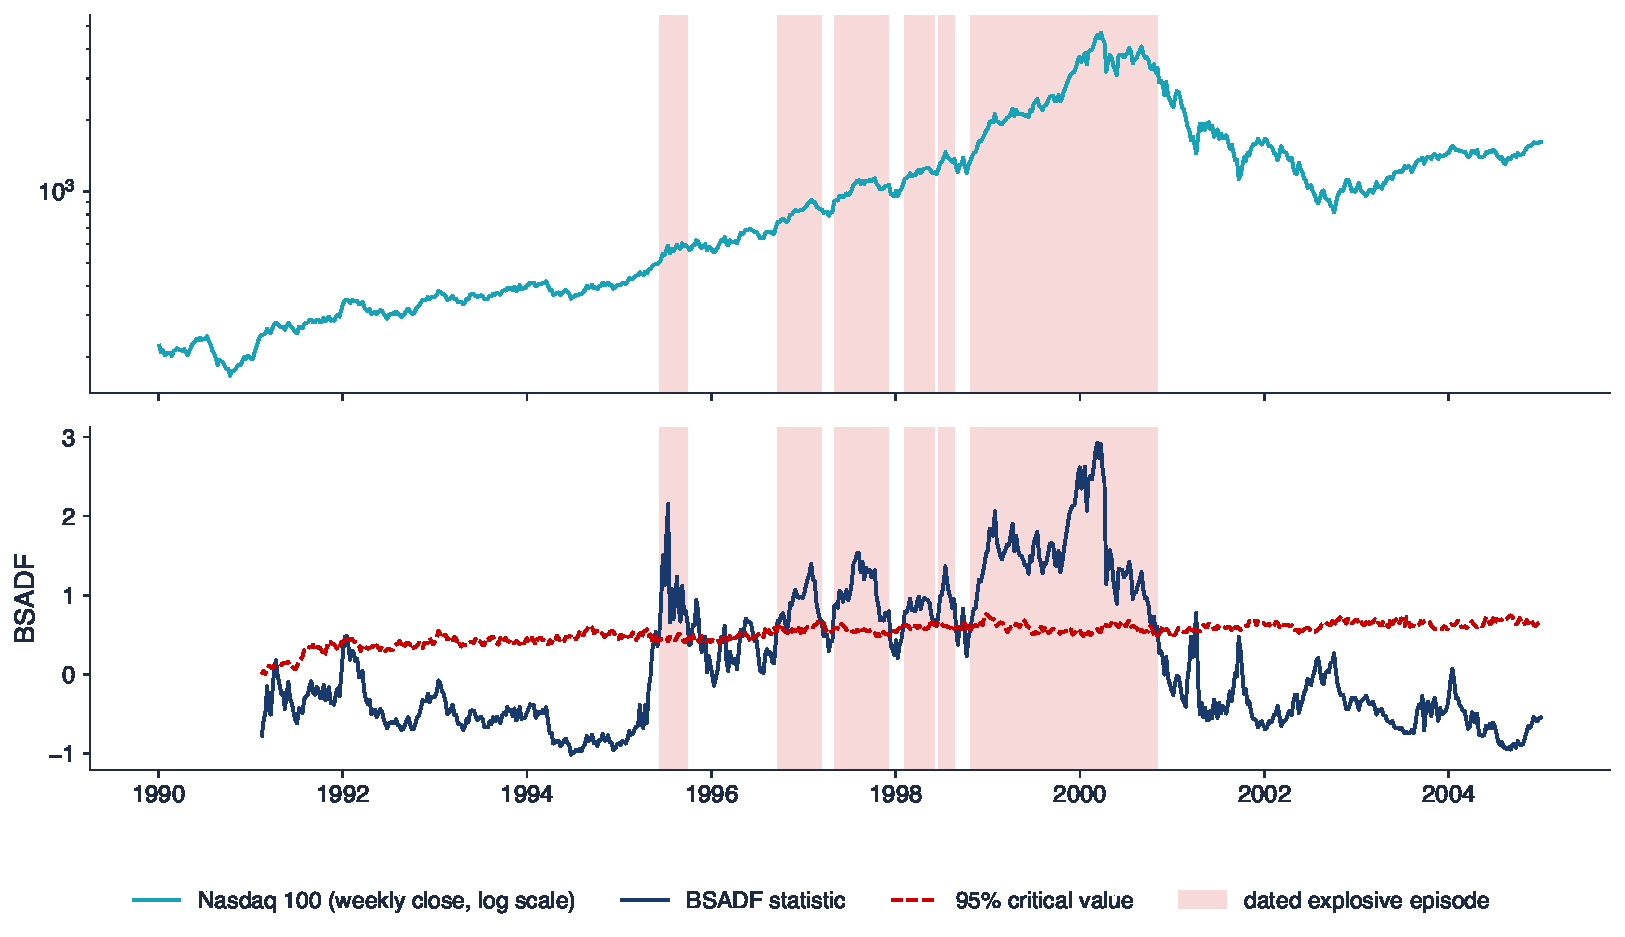
\includegraphics[width=0.97\textwidth,height=0.62\textheight,keepaspectratio]{tsa_ch13_psy_ndx.pdf}
\end{center}
\vspace{-0.25cm}
\begin{itemize}
    \item Top: weekly close, log scale; bottom: BSADF and its 95\% critical values (Monte Carlo, 1000 random walks); shaded: dated episodes (at least 7 weeks above the critical value)
\end{itemize}
\quantlet{TSA\_ch13\_explosive\_roots}{\qlurl{TSA_ch13_explosive_roots}}
\end{frame}

\begin{frame}{Interpreting the Nasdaq 100 tests}
\itemsize{\small}
\begin{itemize}
    \item Whole-sample ADF $-1.27$ (95\% critical value $-0.13$): no evidence
    \begin{itemize}
        \item SADF 2.72 (critical value 1.48) and GSADF 2.92 (critical value 2.28): explosive behaviour
        \item the crash of 2000--2002 hides the bubble from a single test on the whole sample
    \end{itemize}
    \item BSADF dates 6 episodes; the longest runs from 23 October 1998 to 3 November 2000 (107 weeks)
    \begin{itemize}
        \item short explosive bursts already from June 1995: the 1990s boom came in waves, as \refPWY\ found
    \end{itemize}
    \item The end date is late: the statistic stays high for months after the peak; the test dates exuberance, it does not announce the crash
\end{itemize}
\end{frame}

\begin{frame}{Bitcoin, BET and Shanghai: dated episodes}
\itemsize{\footnotesize}
\begin{center}
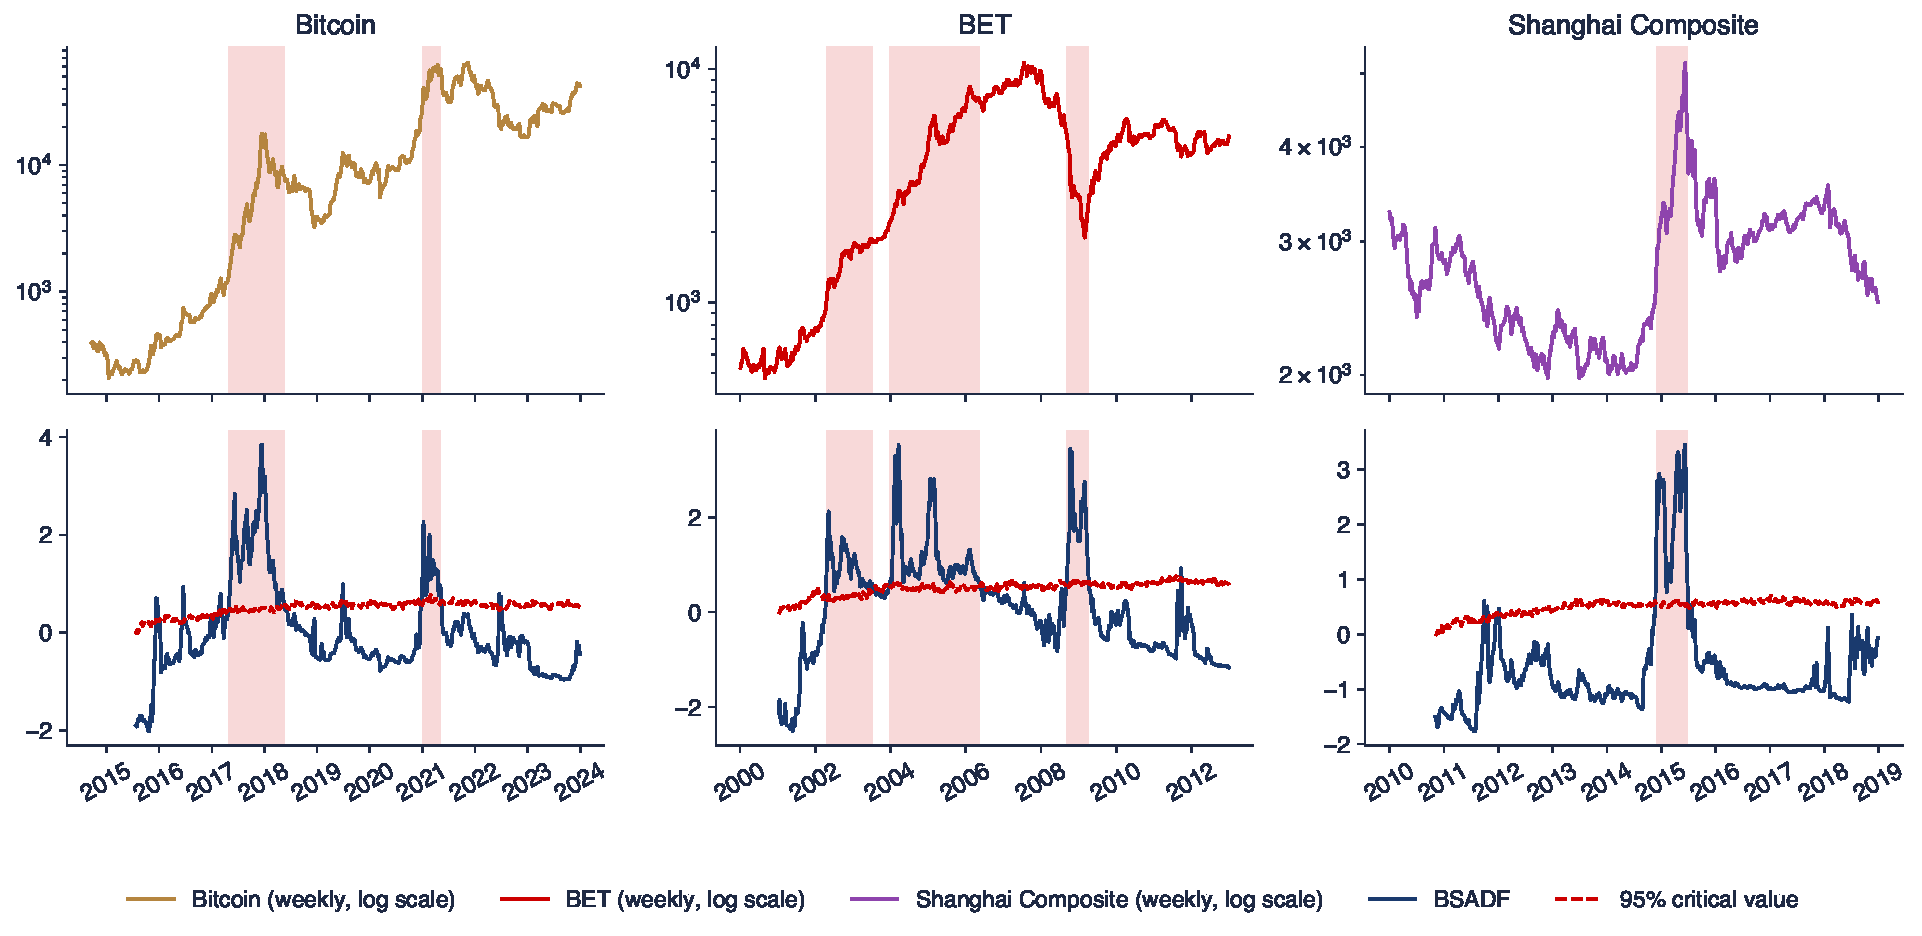
\includegraphics[width=0.97\textwidth,height=0.62\textheight,keepaspectratio]{tsa_ch13_psy_panel.pdf}
\end{center}
\vspace{-0.25cm}
\begin{itemize}
    \item Weekly log closes; top: price with the dated episodes; bottom: BSADF and its 95\% critical values; Bitcoin 2014--2023, BET 2000--2012, Shanghai Composite 2010--2018
\end{itemize}
\quantlet{TSA\_ch13\_explosive\_roots}{\qlurl{TSA_ch13_explosive_roots}}
\end{frame}

\begin{frame}{Interpreting the three markets}
\itemsize{\small}
\begin{itemize}
    \item GSADF: Bitcoin 3.85, BET 3.53, Shanghai 3.46; all above their 95\% critical values (about 2.18)
    \begin{itemize}
        \item Bitcoin: April 2017 -- May 2018 and January 2021 -- May 2021; Shanghai: November 2014 -- June 2015
    \end{itemize}
    \item BET: the explosive phase is December 2003 -- May 2006, not the run-up to July 2007, which was strong but not explosive
    \begin{itemize}
        \item the BET flag of September 2008 -- April 2009 is the collapse: an \textbf{accelerating fall} also gives $\hat\delta > 0$; always read the dates against the price chart
    \end{itemize}
    \item The Bitcoin 2017 episode lasts until May 2018, again well after the peak
\end{itemize}
\end{frame}

\begin{frame}{Limits of the explosive-root tests}
\itemsize{\small}
\begin{itemize}
    \item \textbf{Fundamentals}
    \begin{itemize}
        \item an explosive price is a bubble only if the fundamentals are not explosive
        \item better: test the price--dividend ratio (\refPSYa\ for the S\&P 500); for Bitcoin there are no dividends at all
    \end{itemize}
    \item \textbf{Volatility}
    \begin{itemize}
        \item changing volatility distorts the size of the test
        \item a wild bootstrap gives robust critical values \refPS
    \end{itemize}
    \item \textbf{Timing}
    \begin{itemize}
        \item BSADF uses only past data, so it can run in real time
        \item but it signals a bubble that is already under way and says nothing about when it ends
        \item the LPPL model of the next section tries to answer exactly this: when?
    \end{itemize}
\end{itemize}
\end{frame}

\begin{frame}{Recap: Rational bubbles and explosive roots}
\itemsize{\small}
\begin{itemize}
    \item A rational bubble grows in expectation at the rate $r$: $E_t[B_{t+1}] = (1+r)B_t$, an explosive process
    \item Right-tailed ADF: $H_1$: $\delta > 0$; SADF and GSADF take the supremum over windows; BSADF dates the episodes
    \item Nasdaq 100, Bitcoin, BET and Shanghai all show explosive episodes; the tests date the run-up, not the crash
\end{itemize}
\end{frame}


%=============================================================================
\section{The LPPL model}
%=============================================================================

\begin{frame}{Crashes as critical points}
\itemsize{\footnotesize}
\begin{columns}[T]
\begin{column}{0.38\textwidth}
\centering
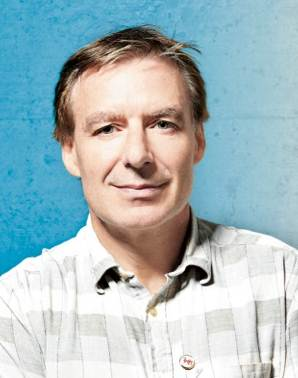
\includegraphics[height=0.36\textheight]{ch13_sornette_2012.jpg}\\[1mm]
\imgcap{Didier Sornette (born 1957)}
\imgcredit{https://commons.wikimedia.org/wiki/File:Didier_Sornette.jpg}{Photo: Didier Sornette (2012); CC BY-SA 3.0 DE; Wikimedia Commons}
\end{column}
\begin{column}{0.6\textwidth}
\begin{itemize}
    \item Physicist, ETH Zürich; with Anders Johansen and Olivier Ledoit he proposed the \textbf{JLS model} \refJLS
    \item Idea: traders imitate their neighbours; imitation creates positive feedback
    \begin{itemize}
        \item rising prices attract buyers, who push prices higher: growth accelerates
        \item the market becomes more and more fragile, like a physical system near a \textbf{critical point} (water near boiling)
    \end{itemize}
    \item The \textbf{critical time} $t_c$
    \begin{itemize}
        \item the most probable moment of the end of the bubble
        \item a crash is likely near $t_c$ but not certain: the bubble may also end with a slow decline
    \end{itemize}
\end{itemize}
\end{column}
\end{columns}
\end{frame}

\begin{frame}{Super-exponential growth}
\itemsize{\footnotesize}
\begin{itemize}
    \item \textbf{Exponential} growth
    \begin{itemize}
        \item constant growth rate, $\ln P(t) = a + g\,t$
        \item $d \ln P/dt = g$
        \item $a$: the initial log price; $g$: the constant growth rate; $d\ln P/dt$: the growth rate of the price at time $t$
        \item a straight line on a log scale
    \end{itemize}
    \item \textbf{Super-exponential} growth
    \begin{itemize}
        \item the growth rate increases with time
        \item on a log scale the curve bends upward
        \item power-law singularity: $\ln P(t) = A + B\,(t_c - t)^m$, with $B < 0$ and $0 < m < 1$
        \item $t_c$: the critical time; $t_c - t$: the time left until it; $A$: the log price reached at $t_c$; $B$: the size of the growth; $m$: the exponent
        \item growth rate $d \ln P/dt = -Bm\,(t_c - t)^{m-1} \to \infty$ as $t \to t_c$, while $\ln P(t_c) = A$ stays finite
    \end{itemize}
    \item Such growth cannot last: it must end at or before $t_c$, a \textbf{finite-time singularity}
\end{itemize}
\end{frame}

\begin{frame}{Exponential and super-exponential growth}
\itemsize{\footnotesize}
\begin{center}
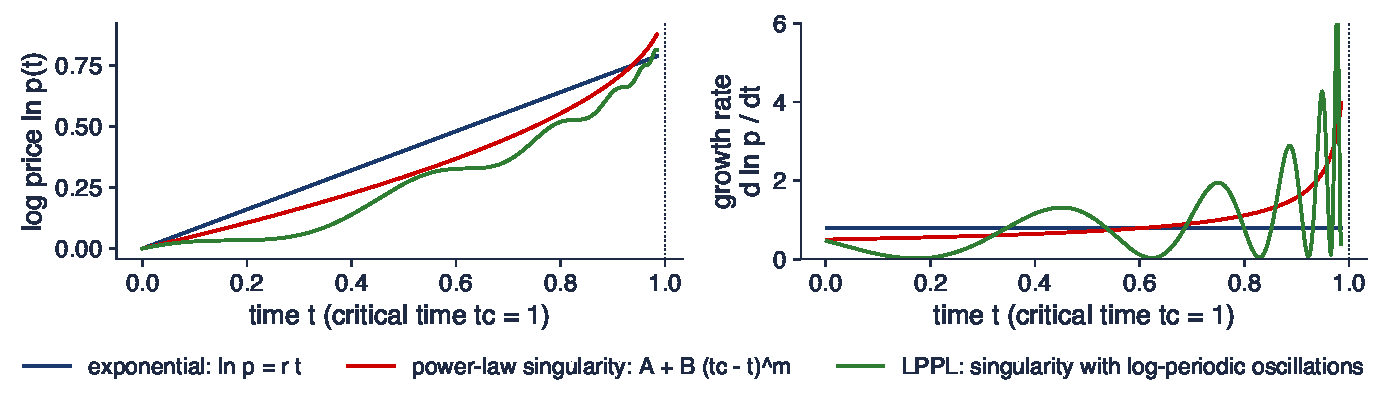
\includegraphics[width=0.97\textwidth,height=0.58\textheight,keepaspectratio]{tsa_ch13_growth.pdf}
\end{center}
\vspace{-0.25cm}
\begin{itemize}
    \item Left: log price; right: its growth rate $d \ln P/dt$; exponential ($g = 0.8$), power-law singularity ($A = 1$, $B = -1$, $m = 0.5$, $t_c = 1$) and the same with log-periodic oscillations
\end{itemize}
\quantlet{TSA\_ch13\_lppl\_model}{\qlurl{TSA_ch13_lppl_model}}
\end{frame}

\begin{frame}{Interpreting the growth paths}
\itemsize{\small}
\begin{itemize}
    \item All three start with similar growth rates: early in a bubble the paths are hard to tell apart
    \item The exponential rate stays at 0.8; the singular rate rises from 0.50 to 0.70 halfway and to 3.98 just before $t_c$
    \item The oscillations ride on the accelerating trend and become faster near $t_c$: the next slides explain why
\end{itemize}
\end{frame}

\begin{frame}{From a crash hazard to the LPPL equation (1/2)}
\itemsize{\footnotesize}
\begin{itemize}
    \item JLS: the relative price change before the crash has three parts
    \begin{itemize}
        \item $dP/P = \mu(t)\,dt + \sigma\,dW - \kappa\, dj$
        \item $\mu(t)\,dt$: the expected growth over a short interval $dt$; $\mu(t)$: the drift, which may change in time
        \item $\sigma\,dW$: the ordinary noise; $W$: a Brownian motion (a continuous random walk); $\sigma$: the volatility
        \item $\kappa\, dj$: the crash; $j$ jumps from 0 to 1 at the crash, which removes a fraction $\kappa$ of the price
    \end{itemize}
    \item \textbf{Hazard rate} $h(t)$
    \begin{itemize}
        \item the probability per unit of time that the crash happens now, given that it has not happened yet
    \end{itemize}
\end{itemize}
\end{frame}

\begin{frame}{From a crash hazard to the LPPL equation (2/2)}
\itemsize{\footnotesize}
\begin{itemize}
    \item No arbitrage: $E[dP] = 0$ $\Rightarrow$ $\mu(t) = \kappa\, h(t)$
    \begin{itemize}
        \item $E[dj] = h(t)\,dt$, so the expected change is zero only if the drift pays for the expected crash loss
        \item the higher the hazard, the faster the price must grow: risk and growth increase together
    \end{itemize}
    \item Imitation near a critical point gives a hazard that rises towards $t_c$ with oscillations
    \begin{itemize}
        \item $h(t) \approx \alpha (t_c - t)^{m-1}[1 + \beta\cos(\omega \ln(t_c - t) - \phi')]$
        \item $\alpha > 0$: the level of the hazard; $(t_c - t)^{m-1}$ grows without bound as $t \to t_c$, since $m < 1$
        \item $\beta$: the relative size of the oscillations; $\omega$: their log-frequency; $\phi'$: their phase
    \end{itemize}
    \item Integrating $\mu(t) = \kappa h(t)$ over time gives the log price on the next slide
\end{itemize}
\end{frame}

\begin{frame}{The LPPL equation}
\itemsize{\footnotesize}
\begin{itemize}
    \item \textbf{Log-periodic power law} (LPPL), for $t < t_c$
    \begin{itemize}
        \item $\quad \ln P(t) = A + B\,(t_c - t)^m + C\,(t_c - t)^m \cos\bigl(\omega \ln(t_c - t) - \phi\bigr)$
    \end{itemize}
\end{itemize}\begin{center}
\scriptsize
\begin{tabular}{lll}
\toprule
\textbf{Parameter} & \textbf{Meaning} & \textbf{Usual range} \\
\midrule
$t_c$ & critical time: most probable end of the bubble & after the last observation \\
$A$ & log price at $t_c$ (if the bubble reached $t_c$) & $A > 0$ \\
$B$ & size of the power-law growth & $B < 0$ (rising price) \\
$m$ & exponent: how fast the growth accelerates & $0 < m < 1$ \\
$C$ & relative size of the oscillations & $|C| < |B|$ \\
$\omega$ & angular log-frequency of the oscillations & $2 \le \omega \le 25$ \\
$\phi$ & phase of the oscillations & $[0, 2\pi)$ \\
\bottomrule
\end{tabular}
\end{center}
\begin{itemize}
    \item Seven parameters: three of them ($t_c$, $m$, $\omega$) enter nonlinearly; $\phi$ disappears in the estimation (Section 4)
\end{itemize}
\end{frame}

\begin{frame}{Log-periodic oscillations}
\itemsize{\small}
\begin{itemize}
    \item $\cos(\omega \ln(t_c - t) - \phi)$ is periodic in $\ln(t_c - t)$, not in $t$: one full cycle each time $\ln(t_c - t)$ changes by $2\pi/\omega$
    \begin{itemize}
        \item successive peaks $t_n$ satisfy $\dfrac{t_c - t_n}{t_c - t_{n+1}} = \lambda = e^{2\pi/\omega}$: the time left to $t_c$ shrinks by the same factor at each cycle
    \end{itemize}
    \item \textbf{Discrete scale invariance}
    \begin{itemize}
        \item the pattern looks the same when time to $t_c$ is rescaled by $\lambda$ (as in a hierarchy of traders, groups, institutions)
    \end{itemize}
    \item Worked example: with $\omega = 8$, $\lambda = e^{2\pi/8} = 2.19$
    \begin{itemize}
        \item if a correction happens 200 days before $t_c$, the next one comes about $200/2.19 \approx 91$ days before $t_c$, then about 42, then 19
        \item $\omega = 6.28$ gives $\lambda = 2.72$; $\omega = 10$ gives $\lambda = 1.87$; the empirical literature reports $\lambda$ near 2 \refSornette
    \end{itemize}
\end{itemize}
\end{frame}

\begin{frame}{The pieces of the LPPL equation}
\itemsize{\footnotesize}
\begin{center}
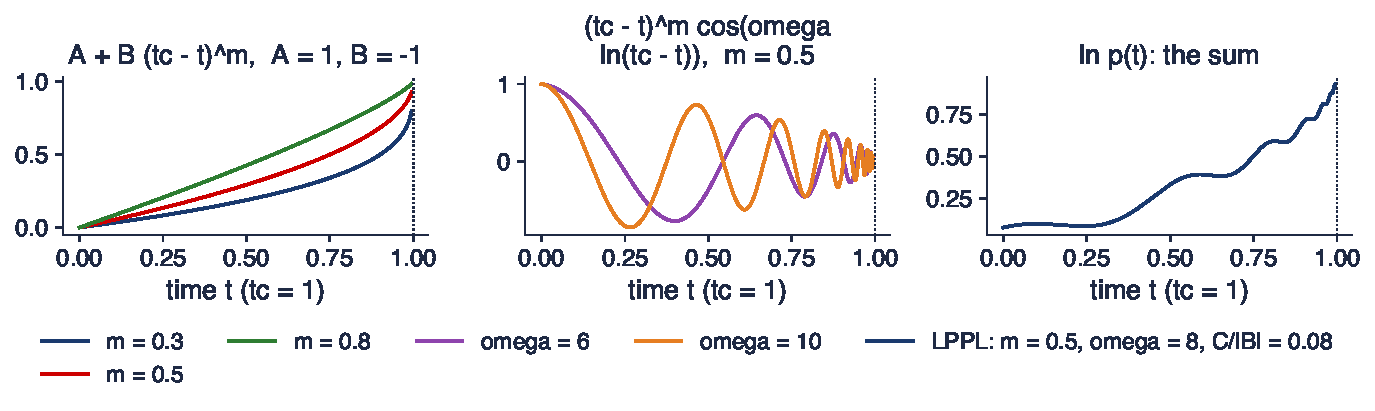
\includegraphics[width=0.97\textwidth,height=0.55\textheight,keepaspectratio]{tsa_ch13_lppl_components.pdf}
\end{center}
\vspace{-0.25cm}
\begin{itemize}
    \item Left: $A + B(t_c - t)^m$ for $m = 0.3, 0.5, 0.8$; middle: the oscillation $(t_c - t)^m \cos(\omega \ln(t_c - t))$ for $\omega = 6$ and $10$; right: the full LPPL path; $t_c = 1$
\end{itemize}
\quantlet{TSA\_ch13\_lppl\_model}{\qlurl{TSA_ch13_lppl_model}}
\end{frame}

\begin{frame}{Interpreting the components}
\itemsize{\small}
\begin{itemize}
    \item A smaller $m$ concentrates the growth close to $t_c$: the curve is flat for a long time, then shoots up
    \begin{itemize}
        \item $m$ close to 1 is almost a straight line: hardly a bubble; $m$ close to 0 is a jump at $t_c$
    \end{itemize}
    \item The oscillation term shrinks with $(t_c - t)^m$ and speeds up: the cycles get shorter by the factor $\lambda$
    \begin{itemize}
        \item a larger $\omega$ gives more cycles before $t_c$
    \end{itemize}
    \item Real run-ups (Section 4) show this mixture: an accelerating trend with corrections that come more and more often
\end{itemize}
\end{frame}

\begin{frame}{Worked example: an LPPL value by hand}
\itemsize{\footnotesize}
\begin{itemize}
    \item Parameters: $A = 8$, $B = -1.2$, $C = 0.08$, $m = 0.5$, $\omega = 8$, $\phi = 0$, $t_c = 2$ (years); compute $\ln P(t)$
    \begin{itemize}
        \item $t = 1$: $t_c - t = 1$, $(t_c - t)^m = 1$, $\ln 1 = 0$, $\cos 0 = 1$: $\ln P = 8 - 1.2 + 0.08 = 6.880$, $P = 973$
        \item $t = 1.75$: $(0.25)^{0.5} = 0.500$, $\ln 0.25 = -1.386$, $\cos(8 \cdot (-1.386)) = 0.095$: $\ln P = 8 - 1.2 \cdot 0.500 + 0.08 \cdot 0.500 \cdot 0.095 = 7.404$, $P = 1642$
        \item $t = 1.99$: $(0.01)^{0.5} = 0.100$, $\cos(8 \cdot (-4.605)) = 0.654$: $\ln P = 7.885$, $P = 2658$
    \end{itemize}
    \item The price rises from 973 to 2658 as $t$ goes from 1 to 1.99 and would reach $e^A = 2981$ at $t_c$; most of the rise comes in the last months
\end{itemize}
\end{frame}

\begin{frame}{Parameter constraints: the filter}
\itemsize{\footnotesize}
\begin{itemize}
    \item A fit is \textbf{qualified} only if it describes a credible bubble (\refSZ, following \refShanghai):
    \begin{itemize}
        \item $B < 0$: rising price; $0.01 \le m \le 0.99$: accelerating growth with a finite price at $t_c$
        \item $2 \le \omega \le 25$: neither too slow nor too fast oscillations; at least 2.5 oscillations in the window, $\frac{\omega}{\pi}\ln\frac{t_c - t_1}{t_c - t_2} \ge 2.5$
        \item $t_2 \le t_c \le t_2 + 0.2\,(t_2 - t_1)$: the end is close, relative to the length of the window $[t_1, t_2]$
        \item damping $\dfrac{m|B|}{\omega|C|} \ge 1$: the hazard rate stays positive
    \end{itemize}
    \item Conditions on the residuals
    \begin{itemize}
        \item every fitted price within 15\% of the observed price; the Lomb periodogram \refLomb\ confirms the log-periodic cycle (level 10\%)
        \item Lomb periodogram: a periodogram for unevenly spaced points, here of the residuals as a function of $\ln(t_c - t)$
        \item the residuals are stationary: the Dickey--Fuller and Phillips--Perron tests of \tsachlink{https://danpele.github.io/Time-Series-Analysis/EN/Courses/chapter3_unit_roots_arima_models.pdf}{Chapter 3} reject a unit root (level 10\%)
    \end{itemize}
\end{itemize}
\end{frame}

\begin{frame}{Recap: The LPPL model}
\itemsize{\small}
\begin{itemize}
    \item Imitation creates a hazard rate that grows towards $t_c$; no arbitrage turns it into super-exponential growth
    \item $\ln P(t) = A + B(t_c - t)^m + C(t_c - t)^m\cos(\omega\ln(t_c - t) - \phi)$, seven parameters
    \item Log-periodic: cycles shrink by $\lambda = e^{2\pi/\omega}$; a fit counts only if it passes the filter
\end{itemize}
\end{frame}


%=============================================================================
\section{Estimation}
%=============================================================================

\begin{frame}{The two-step method of Filimonov and Sornette (1/2)}
\itemsize{\footnotesize}
\begin{itemize}
    \item Least squares over seven parameters has many local minima; \refFS\ reduce the search to three parameters
    \begin{itemize}
        \item $\min \mathrm{SSR} = \sum_{t=t_1}^{t_2} [\ln P_t - \mathrm{LPPL}(t)]^2$; SSR: the sum of squared residuals over the window $[t_1, t_2]$
        \item $\mathrm{LPPL}(t)$: the right-hand side of the LPPL equation
    \end{itemize}
    \item Expand the cosine, with $\tau = t_c - t$
    \begin{itemize}
        \item $C\cos(\omega\ln\tau - \phi) = C_1\cos(\omega\ln\tau) + C_2\sin(\omega\ln\tau)$, where $C_1 = C\cos\phi$, $C_2 = C\sin\phi$
    \end{itemize}
    \item The LPPL equation becomes linear in $A$, $B$, $C_1$, $C_2$
    \begin{itemize}
        \item $\ln P(t) = A + B\,f_t + C_1\,g_t + C_2\,h_t$
        \item $f_t = \tau^m$, $g_t = \tau^m\cos(\omega\ln\tau)$, $h_t = \tau^m\sin(\omega\ln\tau)$: known numbers once $t_c$, $m$, $\omega$ are fixed
    \end{itemize}
\end{itemize}
\end{frame}

\begin{frame}{The two-step method of Filimonov and Sornette (2/2)}
\itemsize{\footnotesize}
\begin{itemize}
    \item \textbf{Step 1} (linear)
    \begin{itemize}
        \item for given $(t_c, m, \omega)$, regress $\ln P_t$ on $(1, f_t, g_t, h_t)$ by OLS
        \item $(\hat A, \hat B, \hat C_1, \hat C_2) = (X'X)^{-1}X'y$; $X$: the matrix with columns $1, f_t, g_t, h_t$; $y$: the vector of $\ln P_t$
        \item this gives the concentrated cost $\mathrm{SSR}(t_c, m, \omega)$, a function of three parameters only
    \end{itemize}
    \item \textbf{Step 2} (nonlinear)
    \begin{itemize}
        \item minimise $\mathrm{SSR}(t_c, m, \omega)$ over the search space
        \item $t_c \in [t_2, t_2 + (t_2 - t_1)/3]$, $m \in [0, 1]$, $\omega \in [1, 50]$
        \item in the code: a grid of $8 \times 8 \times 16$ points, then the Nelder--Mead simplex from the best grid point
    \end{itemize}
    \item At the end: $C = \sqrt{C_1^2 + C_2^2}$ and $\phi = \operatorname{atan2}(C_2, C_1)$
    \begin{itemize}
        \item $\operatorname{atan2}(C_2, C_1)$: the angle of the point $(C_1, C_2)$, in $(-\pi, \pi]$
    \end{itemize}
\end{itemize}
\end{frame}

\begin{frame}{The cost landscape}
\itemsize{\footnotesize}
\begin{center}
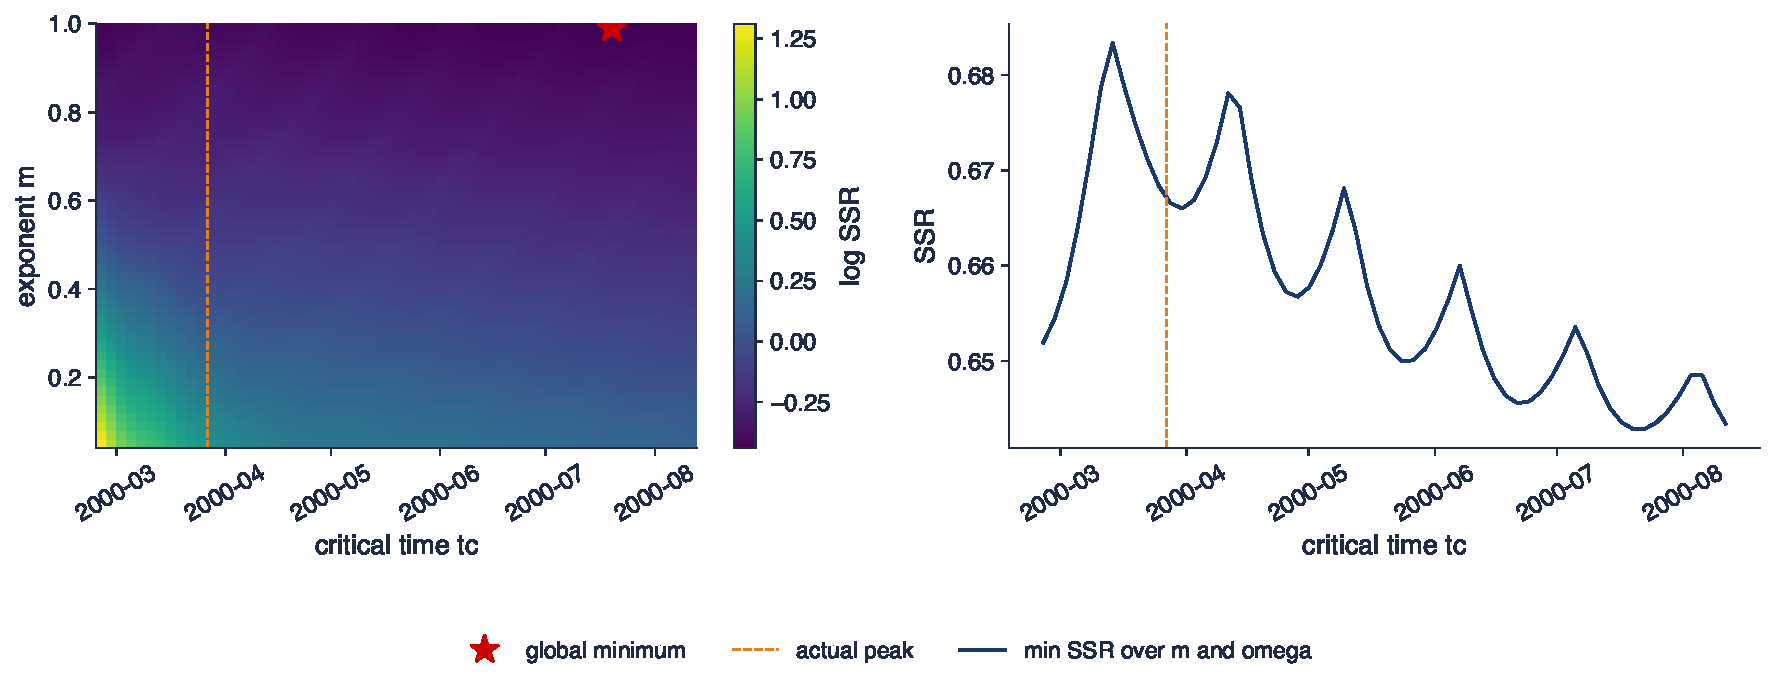
\includegraphics[width=0.97\textwidth,height=0.56\textheight,keepaspectratio]{tsa_ch13_cost.pdf}
\end{center}
\vspace{-0.25cm}
\begin{itemize}
    \item Nasdaq 100, window from the low of October 1998 to 30 days before the peak
    \begin{itemize}
        \item left: $\log \mathrm{SSR}$ over $(t_c, m)$, minimised over $\omega \in [2, 25]$ (135\,360 grid points, with the linear step solved at each point)
        \item right: the minimum over $m$ and $\omega$ as a function of $t_c$
    \end{itemize}
\end{itemize}
\quantlet{TSA\_ch13\_estimation}{\qlurl{TSA_ch13_estimation}}
\end{frame}

\begin{frame}{Interpreting the cost landscape}
\itemsize{\small}
\begin{itemize}
    \item The profile over $t_c$ has 5 local minima: an optimiser started at a different $t_c$ can end in a different valley
    \begin{itemize}
        \item the waves come from the oscillation term: shifting $t_c$ shifts the phase of the cycles
    \end{itemize}
    \item The landscape is flat: the worst and the best $t_c$ differ by only 6.3\% in SSR
    \begin{itemize}
        \item the global minimum is at $m$ near 1 and $t_c$ = 19 July 2000, far after the actual peak: the data barely identify $t_c$
    \end{itemize}
    \item Lesson: one LPPL fit is never enough; we need many windows and the filter (Section 5)
\end{itemize}
\end{frame}

\begin{frame}{Worked example: the Shanghai fit at the end of the window}
\itemsize{\footnotesize}
\begin{itemize}
    \item Shanghai Composite, window 20 March 2014 -- 13 May 2015 (281 days); estimates: $t_c = 2015.428$ (6 June 2015), $m = 0.392$, $\omega = 5.50$
    \begin{itemize}
        \item step 1 gives $\hat A = 8.893$, $\hat B = -1.270$, $\hat C_1 = 0.020$, $\hat C_2 = 0.074$, so $\hat C = 0.076$
    \end{itemize}
    \item At $t_2 = 2015.361$ (years): $\tau = t_c - t_2 = 0.067$, $\tau^m = 0.347$, $\ln\tau = -2.702$
    \begin{itemize}
        \item $\cos(\omega\ln\tau) = -0.656$, $\sin(\omega\ln\tau) = -0.754$
        \item $\widehat{\ln P} = 8.893 + (-0.440) + (-0.024) = 8.429$; observed $\ln P = 8.384$
    \end{itemize}
    \item In levels: fitted 4579 against observed 4376, an error of 4.7\%; the three terms are the level $A$, the power-law growth and the oscillation
\end{itemize}
\end{frame}

\begin{frame}{LPPL fits 30 days before the peak}
\itemsize{\footnotesize}
\begin{center}
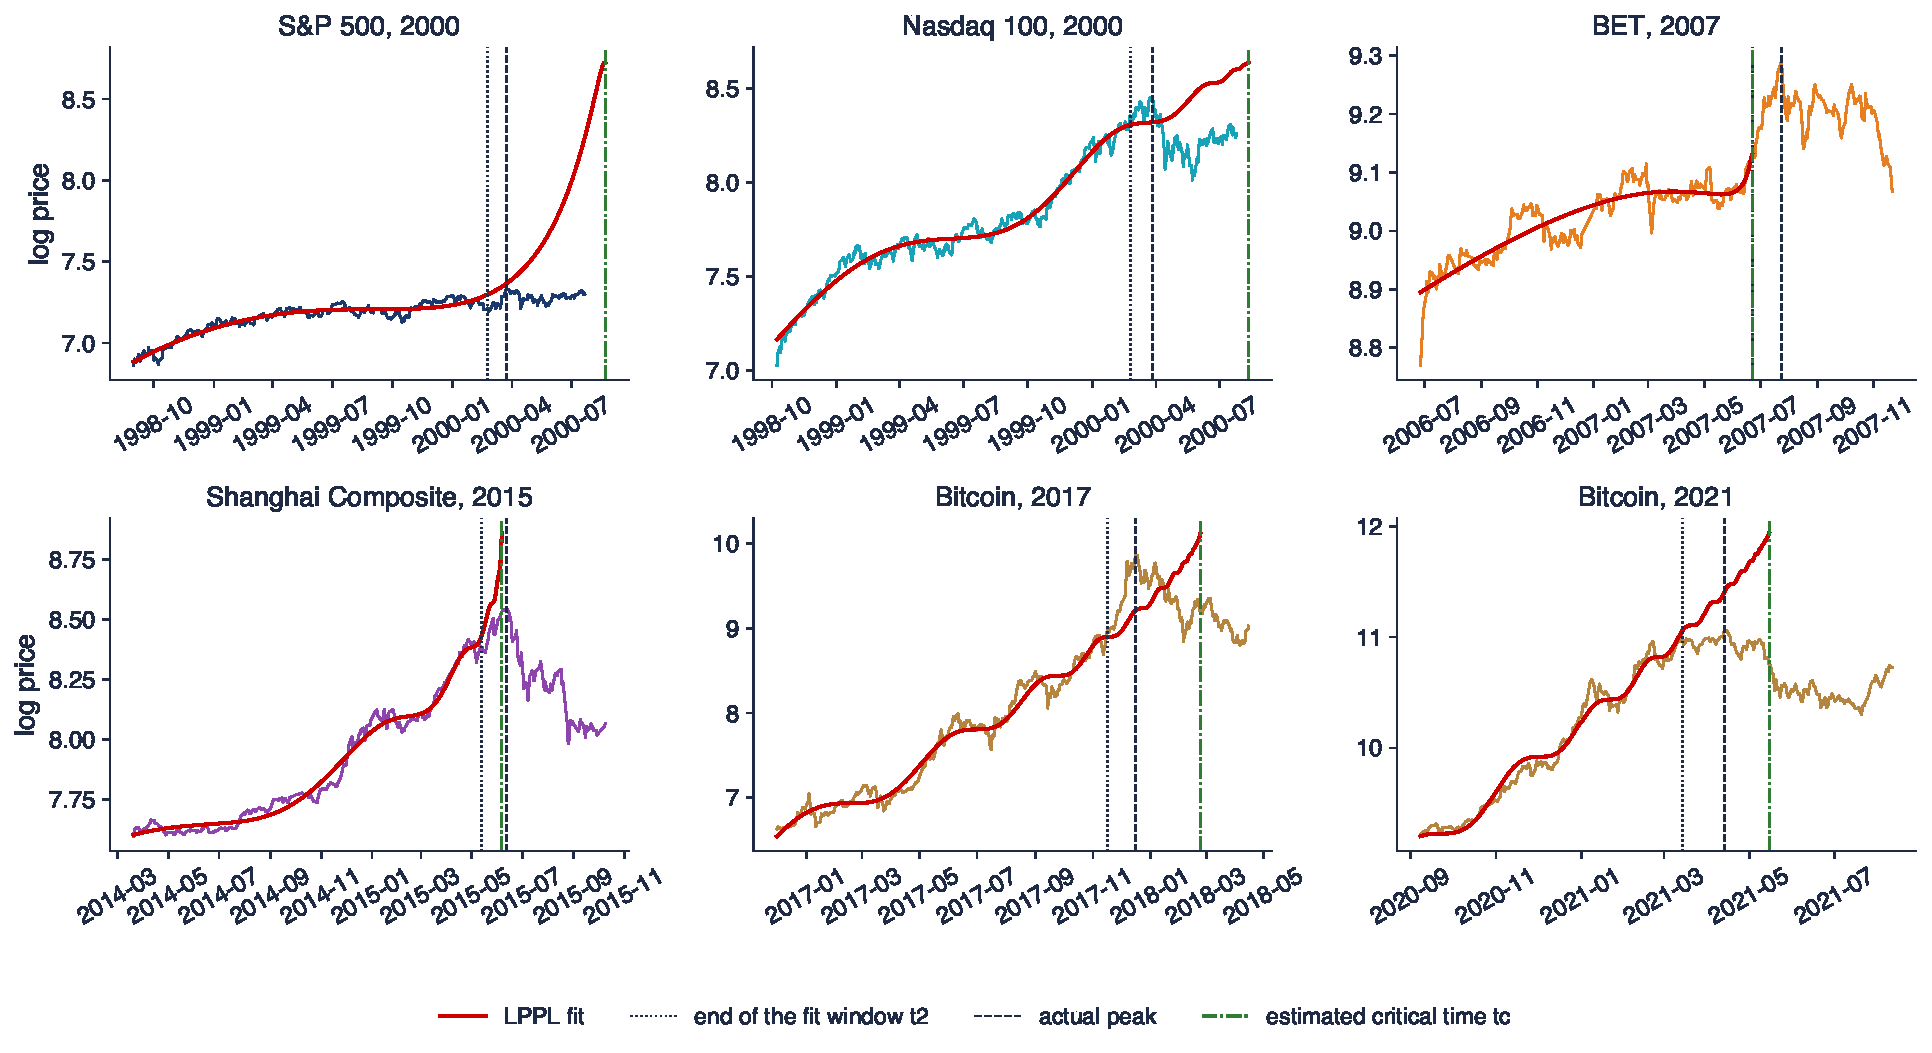
\includegraphics[width=0.97\textwidth,height=0.64\textheight,keepaspectratio]{tsa_ch13_fits.pdf}
\end{center}
\vspace{-0.25cm}
\begin{itemize}
    \item Window: from the low before the run-up to 30 calendar days before the peak; the fitted path is extended to the estimated $t_c$; data after the window are shown only for comparison
\end{itemize}
\quantlet{TSA\_ch13\_estimation}{\qlurl{TSA_ch13_estimation}}
\end{frame}

\begin{frame}{Interpreting the six fits}
\itemsize{\footnotesize}
\begin{center}
\scriptsize
\begin{tabular}{lllrrrll}
\toprule
\textbf{Episode} & $t_2$ & $\hat t_c$ & \textbf{Days to peak} & $\hat m$ & $\hat\omega$ & \textbf{Param.} & \textbf{All} \\
\midrule
S\&P 500, 2000 & 23 February 2000 & 21 August 2000 & +150 & 1.00 & 1.0 & no & no \\
Nasdaq 100, 2000 & 25 February 2000 & 11 August 2000 & +137 & 1.00 & 5.9 & no & no \\
BET, 2007 & 22 June 2007 & 22 June 2007 & $-$32 & 0.69 & 1.0 & no & no \\
Shanghai Composite, 2015 & 13 May 2015 & 6 June 2015 & $-$6 & 0.39 & 5.5 & yes & yes \\
Bitcoin, 2017 & 16 November 2017 & 22 February 2018 & +68 & 0.71 & 14.1 & no & no \\
Bitcoin, 2021 & 14 March 2021 & 15 May 2021 & +32 & 0.82 & 17.4 & no & no \\
\bottomrule
\end{tabular}
\end{center}
\begin{itemize}
    \item Days to peak: $\hat t_c$ minus the actual peak; Param.: the fit passes the parameter conditions; All: it also passes the residual conditions
    \item Only Shanghai passes the whole filter, with $\hat t_c$ within a week of the peak; S\&P 500 and Nasdaq 100 hit the boundary $m = 1$: no super-exponential growth in these windows
    \item Bitcoin fails the 15\% error condition: its daily swings are too large for one smooth path
\end{itemize}
\end{frame}

\begin{frame}{Recap: Estimation}
\itemsize{\small}
\begin{itemize}
    \item Four linear parameters by OLS, three nonlinear ones ($t_c$, $m$, $\omega$) by search: the method of \refFS
    \item The cost surface is rugged and flat in $t_c$: the critical time is weakly identified
    \item One window, one fit: only one of six episodes gives a fully qualified fit 30 days before the peak
\end{itemize}
\end{frame}


%=============================================================================
\section{Confidence from many windows}
%=============================================================================

\begin{frame}{The LPPLS confidence indicator}
\itemsize{\small}
\begin{itemize}
    \item So far $t_1$ was the low before the run-up, a date known only \textbf{after} the bubble; in real time the start is unknown
    \begin{itemize}
        \item remedy: for each end date $t_2$ (today), fit LPPL on 29 windows $[t_2 - L, t_2]$, $L = 750, 725, \dots, 50$ trading days \refSZ
    \end{itemize}
    \item Indicator $=$ share of the windows ending at $t_2$ whose fit is qualified \refShanghai; 0: no window sees a bubble, 1: all do
    \begin{itemize}
        \item LPPLS (LPPL singularity) is the name used for this indicator; the equation is the same
    \end{itemize}
    \item Two versions in this chapter
    \begin{itemize}
        \item \textbf{parameter conditions}: $B$, $m$, $\omega$, $t_c$, oscillations, damping
        \item \textbf{all conditions}: also the 15\% error, the Lomb test and stationary residuals (\refSZ)
    \end{itemize}
    \item Computed only with data up to $t_2$: a real-time indicator; an alarm when it exceeds a threshold fixed in advance (here 0.2)
\end{itemize}
\end{frame}

\begin{frame}{Many windows, one end date}
\itemsize{\footnotesize}
\begin{center}
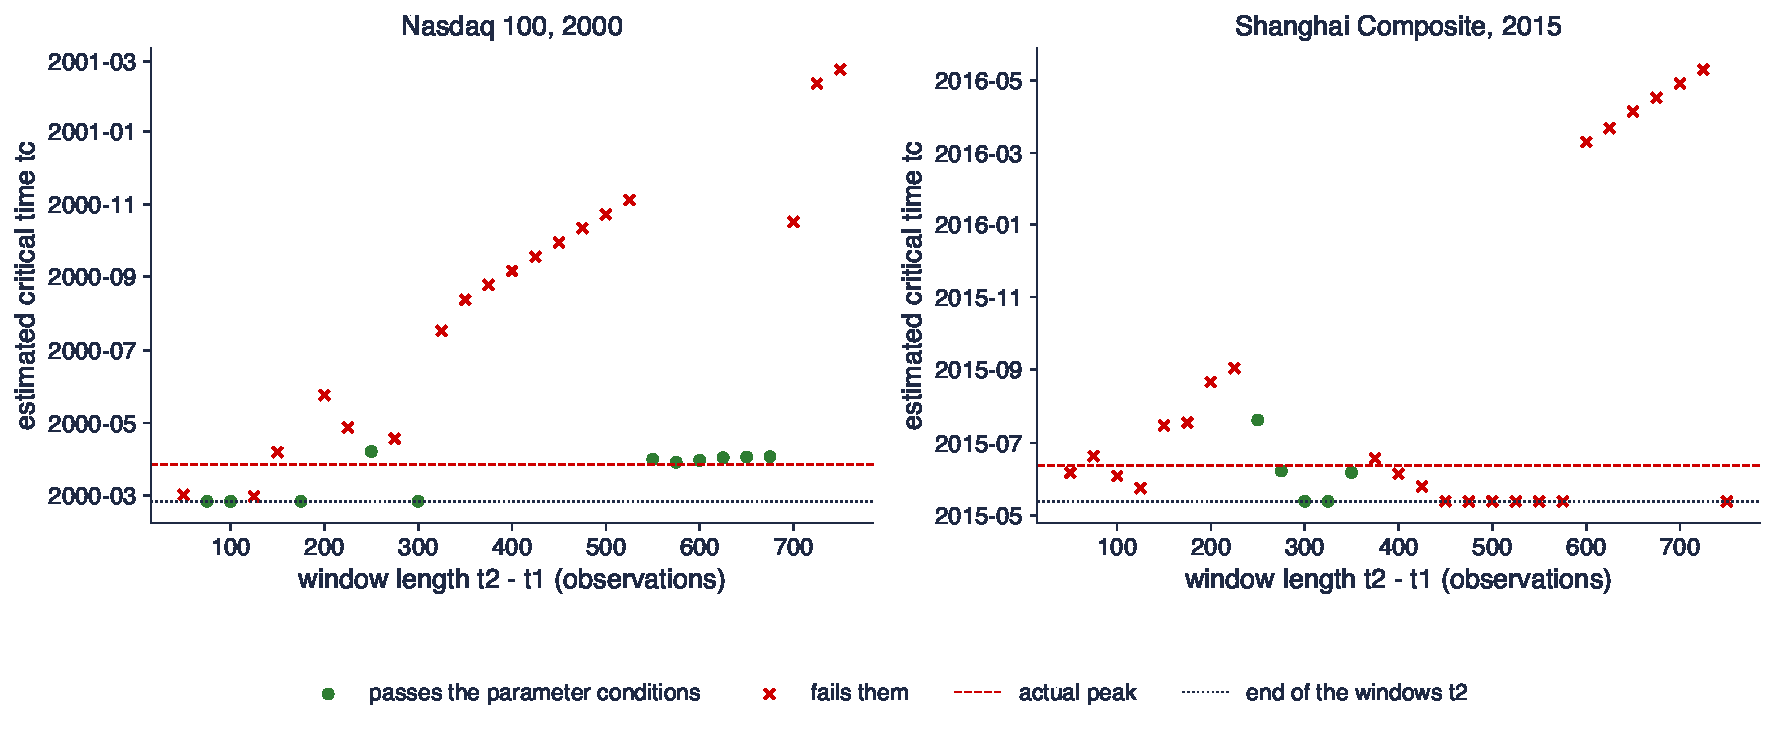
\includegraphics[width=0.97\textwidth,height=0.6\textheight,keepaspectratio]{tsa_ch13_windows.pdf}
\end{center}
\vspace{-0.25cm}
\begin{itemize}
    \item Estimated $t_c$ for each of the 29 windows ending 30 days before the peak; green dots: the fit passes the parameter conditions; red crosses: it fails them
\end{itemize}
\quantlet{TSA\_ch13\_confidence}{\qlurl{TSA_ch13_confidence}}
\end{frame}

\begin{frame}{Interpreting the windows}
\itemsize{\small}
\begin{itemize}
    \item Nasdaq 100 (end 25 February 2000): 11 of 29 windows pass the parameter conditions, 1 the whole filter
    \begin{itemize}
        \item qualified $\hat t_c$: median 30 March 2000, 10\%--90\% range 25 February 2000 -- 2 April 2000; actual peak 27 March 2000
    \end{itemize}
    \item Shanghai (end 13 May 2015): 5 of 29 pass the parameter conditions; median $\hat t_c$ 6 June 2015, actual peak 12 June 2015
    \begin{itemize}
        \item the condition on $m$ fails most often: only 41\% of the Shanghai windows have $0.01 \le m \le 0.99$
    \end{itemize}
    \item Short windows put $t_c$ right after $t_2$; long windows spread it out: the window length is a hidden modelling choice
\end{itemize}
\end{frame}

\begin{frame}{The indicator around four peaks (1/2)}
\itemsize{\footnotesize}
\begin{center}
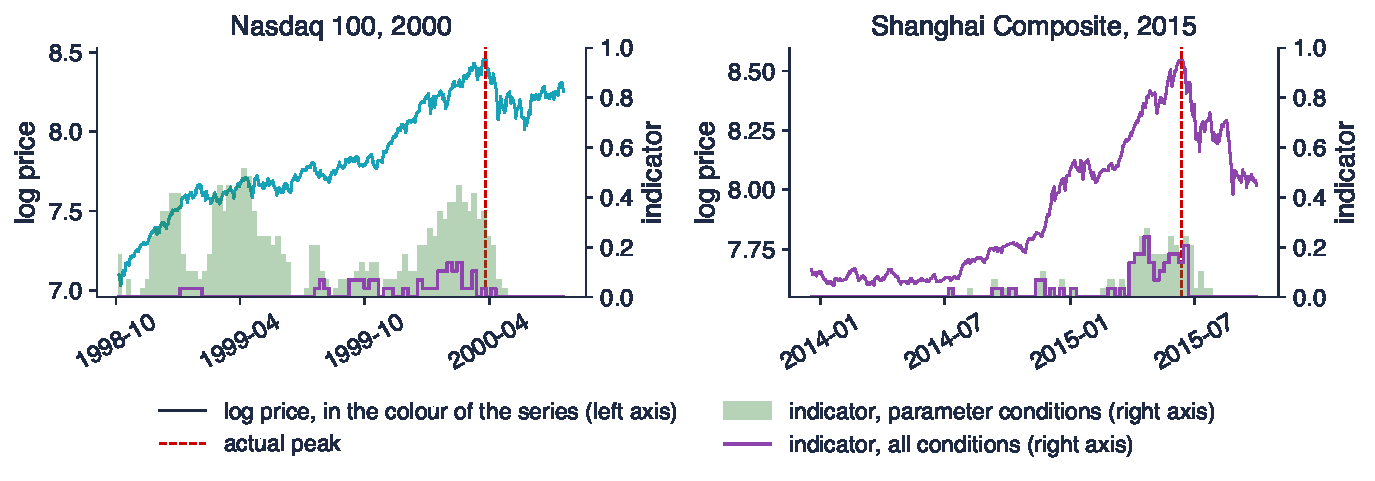
\includegraphics[width=0.97\textwidth,height=0.64\textheight,keepaspectratio]{tsa_ch13_ci.pdf}
\end{center}
\vspace{-0.25cm}
\begin{itemize}
    \item Log price (left axis) and the indicator (right axis) every 5 trading days, from 18 months before to 4 months after the peak
    \begin{itemize}
        \item green area: parameter conditions; purple line: all conditions
    \end{itemize}
\end{itemize}
\quantlet{TSA\_ch13\_confidence}{\qlurl{TSA_ch13_confidence}}
\end{frame}

\begin{frame}{The indicator around four peaks (2/2)}
\itemsize{\footnotesize}
\begin{center}
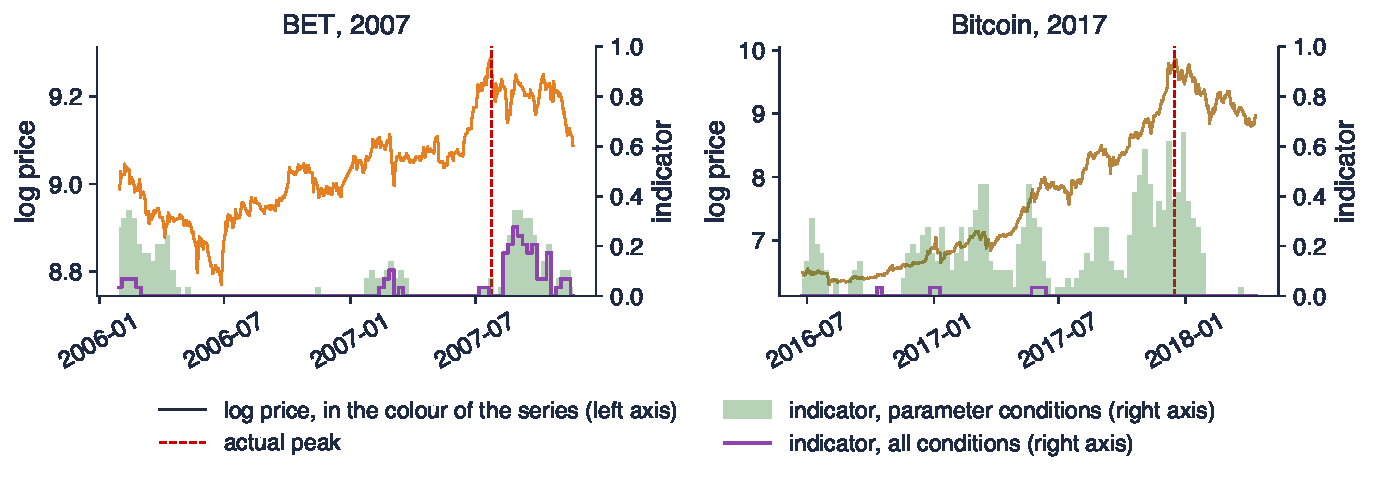
\includegraphics[width=0.97\textwidth,height=0.64\textheight,keepaspectratio]{tsa_ch13_ci_b.pdf}
\end{center}
\vspace{-0.25cm}
\begin{itemize}
    \item The same layout and colours as in (1/2), for the BET (2007) and Bitcoin (2017); Bitcoin: one value every 7 days
\end{itemize}
\quantlet{TSA\_ch13\_confidence}{\qlurl{TSA_ch13_confidence}}
\end{frame}

\begin{frame}{Interpreting the indicator}
\itemsize{\small}
\begin{itemize}
    \item Nasdaq 100: the parameter version reaches 0.52 on 7 April 1999, a year before the peak, and rises again in the last months; the full version stays below 0.14
    \begin{itemize}
        \item Shanghai: both versions rise in the two months before the peak (maximum 0.24 on 22 April 2015)
    \end{itemize}
    \item BET: the strongest full-filter signal, 0.28, comes on 28 August 2007, after the peak: the fits then describe the last part of the run-up, not the future
    \begin{itemize}
        \item Bitcoin 2017: the parameter version peaks at 0.66 on 29 December 2017; the full version is almost always 0 (the 15\% error condition)
    \end{itemize}
    \item The indicator does light up in bubbles, but early, late and with gaps; the choice of filter changes the picture
\end{itemize}
\end{frame}

\begin{frame}{The critical time moves with the data}
\itemsize{\footnotesize}
\begin{center}
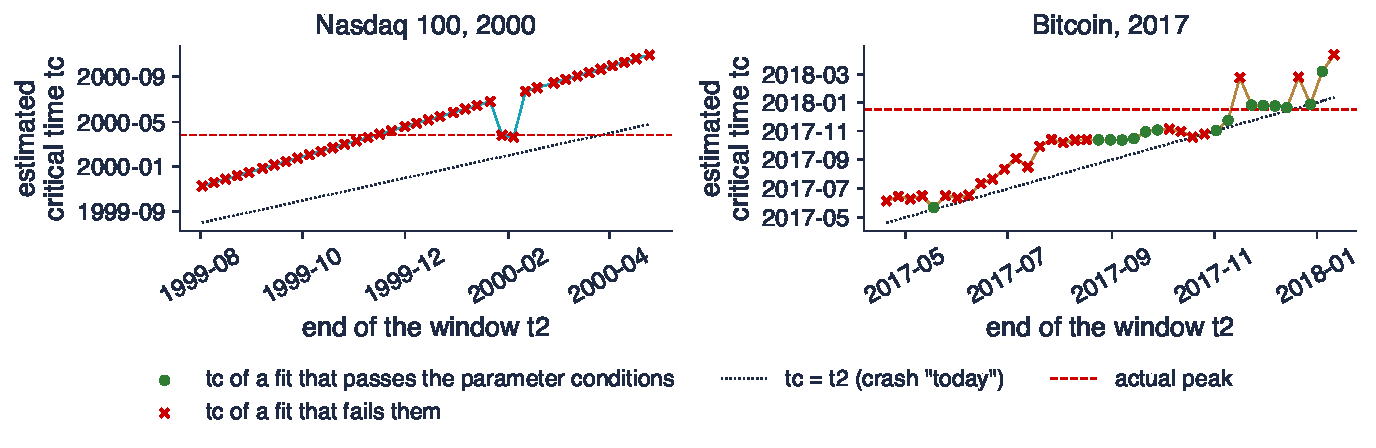
\includegraphics[width=0.97\textwidth,height=0.6\textheight,keepaspectratio]{tsa_ch13_tc_path.pdf}
\end{center}
\vspace{-0.25cm}
\begin{itemize}
    \item Window start fixed at the low before the run-up; the end $t_2$ moves from 8 months before to 1 month after the peak (weekly); each point: the $\hat t_c$ of the fit ending at $t_2$
\end{itemize}
\quantlet{TSA\_ch13\_confidence}{\qlurl{TSA_ch13_confidence}}
\end{frame}

\begin{frame}{Interpreting the moving critical time}
\itemsize{\small}
\begin{itemize}
    \item Nasdaq 100: over 38 end dates $\hat t_c$ ranges from 9 November 1999 to 30 October 2000 (356 days); none of these fits passes the parameter conditions
    \begin{itemize}
        \item Bitcoin 2017: range 21 May 2017 -- 12 April 2018; 38\% of the fits pass; median error 65 days
    \end{itemize}
    \item Many points lie close to the line $t_c = t_2$: the fit often says ``the end is now'', week after week
    \begin{itemize}
        \item a forecast that keeps moving with the data is a description of the past, not a prediction
    \end{itemize}
    \item Picking, after the crash, the one window whose $\hat t_c$ was right is \textbf{look-ahead bias}
\end{itemize}
\end{frame}

\begin{frame}{Recap: Confidence from many windows}
\itemsize{\small}
\begin{itemize}
    \item The start of a bubble is unknown: fit 29 windows for each end date
    \item Indicator = share of qualified windows; it depends strongly on the filter
    \item $\hat t_c$ moves with the end of the data: report its spread over windows, never one value
\end{itemize}
\end{frame}


%=============================================================================
\section{An honest evaluation of crash prediction}
%=============================================================================

\begin{frame}{Traps in evaluating crash predictions}
\itemsize{\small}
\begin{itemize}
    \item \textbf{Look-ahead bias}
    \begin{itemize}
        \item using information from after $t_2$
        \item choosing $t_1$ at the low of the run-up, the episodes after the crash, or the filter after seeing the results
    \end{itemize}
    \item \textbf{Selection}
    \begin{itemize}
        \item studying only the bubbles that burst
        \item the run-ups that did not end in a crash are forgotten
    \end{itemize}
    \item \textbf{False alarms and base rates}
    \begin{itemize}
        \item an alarm is useful only if a crash is \textbf{more likely after an alarm} than on an ordinary day
        \item the comparison: $P(\text{crash} \mid \text{alarm})$ against $P(\text{crash})$, the unconditional frequency
    \end{itemize}
    \item A fair test fixes everything in advance (windows, filter, threshold, the definition of a crash) and runs over the whole sample
\end{itemize}
\end{frame}

\begin{frame}{Alarms over the whole sample (1/2)}
\itemsize{\footnotesize}
\begin{center}
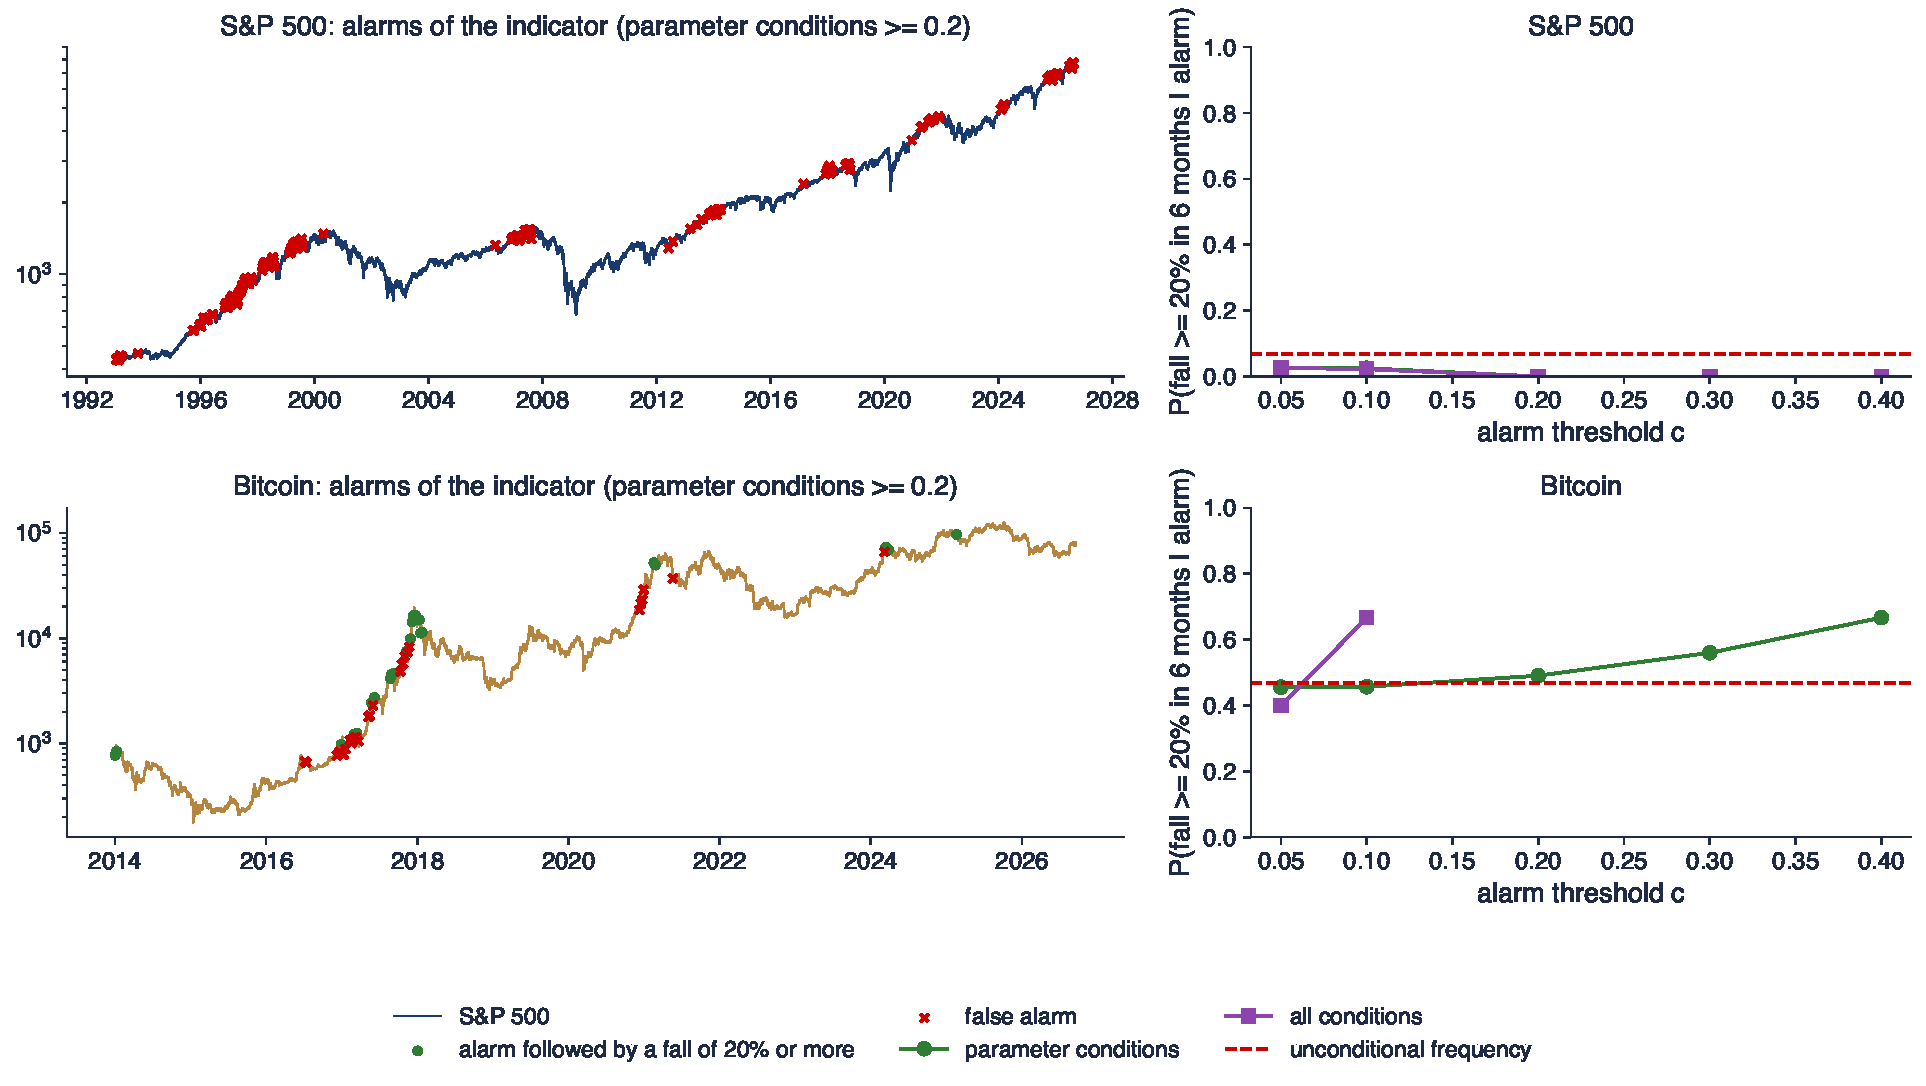
\includegraphics[width=0.97\textwidth,height=0.62\textheight,keepaspectratio]{tsa_ch13_eval.pdf}
\end{center}
\vspace{-0.25cm}
\begin{itemize}
    \item S\&P 500: indicator every 5 trading days, January 1993 -- September 2026
    \begin{itemize}
        \item a crash: a fall of at least 20\% within 182 days after the alarm; right: hit rate by threshold
    \end{itemize}
\end{itemize}
\quantlet{TSA\_ch13\_evaluation}{\qlurl{TSA_ch13_evaluation}}
\end{frame}

\begin{frame}{Alarms over the whole sample (2/2)}
\itemsize{\footnotesize}
\begin{center}
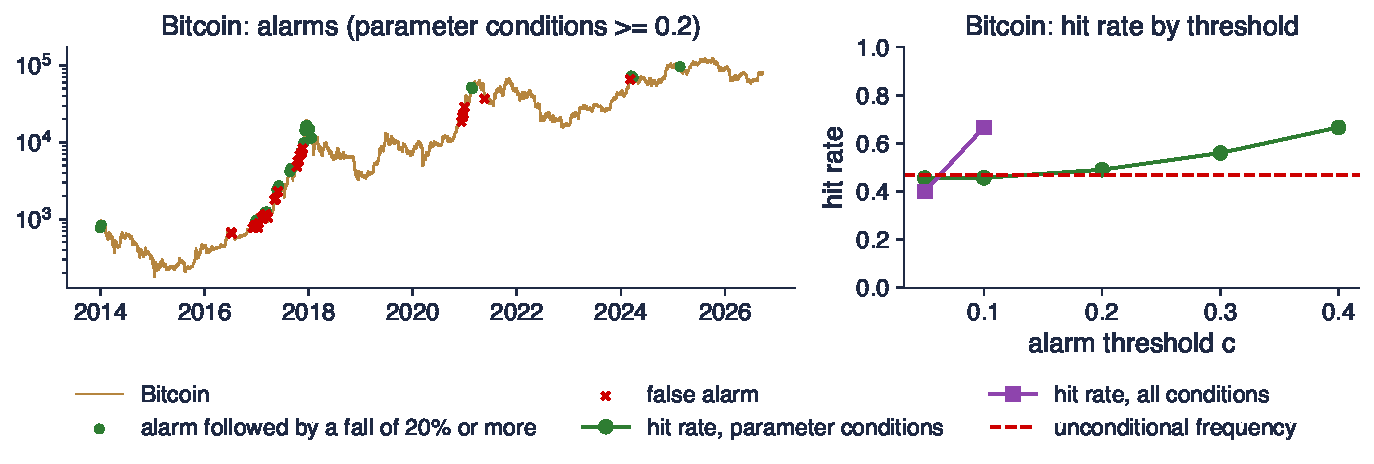
\includegraphics[width=0.97\textwidth,height=0.62\textheight,keepaspectratio]{tsa_ch13_eval_btc.pdf}
\end{center}
\vspace{-0.25cm}
\begin{itemize}
    \item Bitcoin: indicator every 7 days, January 2014 -- September 2026
    \begin{itemize}
        \item hit rate: the share of the alarm dates followed by a crash; dashed line: the unconditional frequency
    \end{itemize}
\end{itemize}
\quantlet{TSA\_ch13\_evaluation}{\qlurl{TSA_ch13_evaluation}}
\end{frame}

\begin{frame}{Interpreting the evaluation}
\itemsize{\small}
\begin{itemize}
    \item S\&P 500: a fall of 20\% within six months follows 7\% of all dates, but 0\% of the alarm dates (threshold 0.2, parameter conditions)
    \begin{itemize}
        \item 20 alarm clusters, none followed by such a fall within six months; the alarms come in calm, steady uptrends
        \item of the 4 drawdowns of 20\% or more since January 1993, 2 had an alarm in the six months before their peak (2007 and 2022), but the falls came later
    \end{itemize}
    \item Bitcoin: base rate 47\%, after an alarm 49\%: almost no gain; 12 of its 14 drawdowns of 20\% had an alarm before the peak
    \begin{itemize}
        \item falls of 20\% are so frequent in Bitcoin that almost any alarm looks ``right''; higher thresholds help a little, on very few dates (56\% at 0.3, on 4\% of the dates)
    \end{itemize}
    \item The indicator says ``this looks like a bubble regime'', not ``the crash comes within six months''
\end{itemize}
\end{frame}

\begin{frame}{The literature on crash prediction}
\itemsize{\small}
\begin{itemize}
    \item Successes reported by the authors of the method
    \begin{itemize}
        \item \refJiang: the Chinese bubbles of 2007 and 2009 diagnosed in advance; \refShanghai: the Shanghai 2015 peak announced before it happened
        \item \refGerlach: Bitcoin's bubbles of 2012--2018 dissected with the confidence indicator
    \end{itemize}
    \item Critical evaluations
    \begin{itemize}
        \item \refFeig: the log-periodic term adds little once the estimation error is taken into account
        \item \refBJ: on many crashes, the LPPL conditions are rarely all met before the crash; parameters are unstable
    \end{itemize}
    \item Our own numbers point the same way: the indicator reacts to strong run-ups, but its timing is loose and its alarms are often false
\end{itemize}
\end{frame}

\begin{frame}{Strengths and limits of LPPL}
\itemsize{\small}
\begin{itemize}
    \item \textbf{Can}
    \begin{itemize}
        \item describe a run-up with accelerating growth and shrinking corrections in a few interpretable parameters
        \item measure ``how bubble-like'' a market is today, across many windows (the indicator)
    \end{itemize}
    \item \textbf{Cannot}
    \begin{itemize}
        \item give the date of a crash: $t_c$ marks the end of the regime
        \item guarantee a crash: the regime may end with a slow decline
        \item tell whether the price is above the fundamental value: that needs fundamentals
    \end{itemize}
    \item Use it with the explosive-root tests, with fundamentals (valuation ratios) and with risk measures such as VaR 1\% (\tsachlink{https://danpele.github.io/Time-Series-Analysis/EN/Courses/chapter5_conditional_volatility_garch.pdf}{Chapter 5}), not alone
\end{itemize}
\end{frame}

\begin{frame}{Recap: An honest evaluation}
\itemsize{\small}
\begin{itemize}
    \item Fix windows, filter, threshold and the definition of a crash before looking at the outcomes
    \item Compare the hit rate after alarms with the base rate; count the false alarms
    \item LPPL describes bubbles well; as a crash-timing tool its record is weak
\end{itemize}
\end{frame}


%=============================================================================
\section{Possible contribution of AI}
%=============================================================================

\begin{frame}{Possible contribution of AI}
\itemsize{\small}
\begin{itemize}
    \item \textbf{Code}
    \begin{itemize}
        \item a first version of the BSADF recursion, of the Filimonov--Sornette two-step fit, of the indicator over many windows
    \end{itemize}
    \item \textbf{Explanation}
    \begin{itemize}
        \item a second explanation of the hazard-rate argument or of log-periodicity, with your own numbers
    \end{itemize}
    \item \textbf{Exploration}
    \begin{itemize}
        \item the indicator on many markets and periods, with different filters, under a protocol fixed in advance
    \end{itemize}
    \item Example prompt
    \begin{itemize}
        \item \aiprompt{Write Python code that fits the LPPL model to the daily log price of the Shanghai Composite between two dates with the Filimonov-Sornette method (OLS for A, B, C1, C2; grid search plus Nelder-Mead for tc, m, omega), checks the filter conditions of Shu and Zhu (2020) and plots the fit.}
    \end{itemize}
\end{itemize}
\end{frame}

\begin{frame}{Checks you must run}
\itemsize{\small}
\begin{itemize}
    \item Simulate an LPPL path with known parameters plus noise and check that the code recovers $t_c$, $m$ and $\omega$
    \item The sign conventions: $B < 0$ for a rising bubble; the test of explosive roots uses the right tail, not the left tail of \tsachlink{https://danpele.github.io/Time-Series-Analysis/EN/Courses/chapter3_unit_roots_arima_models.pdf}{Chapter 3}
    \item Critical values: SADF and GSADF need their own simulated critical values, not the Dickey--Fuller table
    \item No look-ahead: every quantity at date $t_2$ must use only data up to $t_2$
    \item A crash ``predicted'' by an AI answer after the fact is not a prediction; ask for the full list of alarms and false alarms
    \item Every cited reference: it must exist; check the DOI
\end{itemize}
\end{frame}


%=============================================================================
\section{Summary}
%=============================================================================

\begin{frame}{Key takeaways}
\itemsize{\small}
\begin{itemize}
    \item A bubble is a price above its fundamental value; a rational bubble must grow explosively
    \item Right-tailed ADF tests (SADF, GSADF, BSADF) detect and date explosive episodes with data up to each date
    \item LPPL: super-exponential growth with log-periodic oscillations ending at a critical time $t_c$
    \item Estimate in two steps (OLS + search over $t_c$, $m$, $\omega$), filter the fits, use many windows
    \item Judge predictions by hit rates against base rates, with all the false alarms: the timing of crashes remains hard
\end{itemize}
\end{frame}

\begin{frame}{Key formulas}
\itemsize{\small}
{\renewcommand{\arraystretch}{1.35}\begin{center}
\footnotesize
\begin{tabular}{ll}
\toprule
\textbf{Quantity} & \textbf{Formula} \\
\midrule
Rational bubble & $P_t = F_t + B_t$, \quad $E_t[B_{t+1}] = (1+r)B_t$ \\
Right-tailed ADF & $\Delta y_t = a + \delta y_{t-1} + \varepsilon_t$, \quad $H_1$: $\delta > 0$ \\
GSADF, BSADF & $\sup_{r_2}\sup_{r_1}\mathrm{ADF}_{r_1}^{r_2}$, \quad $\mathrm{BSADF}(r_2) = \sup_{r_1}\mathrm{ADF}_{r_1}^{r_2}$, \quad $r_0 = 0.01 + 1.8/\sqrt T$ \\
LPPL & $\ln P(t) = A + B(t_c - t)^m + C(t_c - t)^m\cos(\omega\ln(t_c - t) - \phi)$ \\
Linear form & $\ln P(t) = A + Bf_t + C_1g_t + C_2h_t$, \quad $C = \sqrt{C_1^2 + C_2^2}$ \\
Scaling ratio & $\lambda = e^{2\pi/\omega}$ \\
Damping & $m|B|/(\omega|C|) \ge 1$ \\
Indicator & share of qualified windows ending at $t_2$ \\
\bottomrule
\end{tabular}
\end{center}
}
\end{frame}

\begin{frame}{Self-assessment (1/2)}
\itemsize{\small}
\begin{itemize}
    \item \textbf{Question}: in a Blanchard--Watson bubble with $r = 1\%$ and $\pi = 0.95$, by how much does the bubble grow in a period in which it survives?
    \begin{itemize}
        \item \textbf{Answer}: by $1.01/0.95 - 1 \approx 6.3\%$; expected lifetime $1/(1 - 0.95) = 20$ periods
    \end{itemize}
    \item \textbf{Question}: a right-tailed ADF on a window gives $\hat\delta = 0.004$ with SE 0.002. Is the window explosive at 5\% if the critical value is 1.5?
    \begin{itemize}
        \item \textbf{Answer}: yes: $t = 0.004/0.002 = 2 > 1.5$; we reject the unit root in favour of an explosive root
    \end{itemize}
    \item \textbf{Question}: why do we use the right tail and not the left tail of \tsachlink{https://danpele.github.io/Time-Series-Analysis/EN/Courses/chapter3_unit_roots_arima_models.pdf}{Chapter 3}?
    \begin{itemize}
        \item \textbf{Answer}: the alternative is $\rho > 1$ (explosive), not $\rho < 1$ (stationary); evidence for it is a large positive $t$
    \end{itemize}
\end{itemize}
\end{frame}

\begin{frame}{Self-assessment (2/2)}
\itemsize{\small}
\begin{itemize}
    \item \textbf{Question}: an LPPL fit gives $\omega = 6.28$. By what factor does the time left to $t_c$ shrink between two corrections?
    \begin{itemize}
        \item \textbf{Answer}: $\lambda = e^{2\pi/6.28} \approx e \approx 2.72$
    \end{itemize}
    \item \textbf{Question}: a fit has $m = 1.0$ at the edge of the search space. Is it a qualified bubble fit?
    \begin{itemize}
        \item \textbf{Answer}: no: the filter needs $m \le 0.99$; $m = 1$ is a linear trend in $t$, not an accelerating one
    \end{itemize}
    \item \textbf{Question}: an indicator gives alarms before 8 of 10 crashes. Is it a good predictor?
    \begin{itemize}
        \item \textbf{Answer}: not yet: we also need the false alarms and the base rate; if alarms are on almost every day, catching 8 crashes is easy
    \end{itemize}
\end{itemize}
\end{frame}

\begin{frame}{Project idea}
\itemsize{\small}
\begin{itemize}
    \item \textbf{Is the BET in a bubble today?} A real-time protocol, fixed before looking at the result
    \begin{itemize}
        \item BSADF on the weekly BET and BET-TR; the indicator of this chapter on the daily BET
        \item the evaluation of Section 6 on the BET since 2000: alarms, false alarms, base rate
    \end{itemize}
    \item Extensions
    \begin{itemize}
        \item the price--earnings ratio instead of the price; Bitcoin and Ethereum together
        \item compare with the regime-switching models of \tsachlink{https://danpele.github.io/Time-Series-Analysis/EN/Courses/chapter10_state_space_kalman_markov_switching.pdf}{Chapter 10}
    \end{itemize}
    \item Further reading on the Bucharest Stock Exchange: \refPeleCrash
    \item Next: \tsachlink{https://danpele.github.io/Time-Series-Analysis/EN/Courses/chapter14_multivariate_garch_models.pdf}{Chapter 14}, multivariate GARCH models
\end{itemize}
\end{frame}


%=============================================================================
\section{References}
%=============================================================================

\begin{frame}{References (1/3)}
\itemsize{\scriptsize}
\begin{itemize}
    \item Blanchard, O. J., \& Watson, M. W. (1982). Bubbles, rational expectations and financial markets. NBER Working Paper 945. \href{https://doi.org/10.3386/w0945}{doi:10.3386/w0945}
    \item Brée, D. S., \& Joseph, N. L. (2013). Testing for financial crashes using the log periodic power law model. \textit{International Review of Financial Analysis}, 30, 287--297. \href{https://doi.org/10.1016/j.irfa.2013.05.005}{doi:10.1016/j.irfa.2013.05.005}
    \item Dickey, D. A., \& Fuller, W. A. (1979). Distribution of the estimators for autoregressive time series with a unit root. \textit{Journal of the American Statistical Association}, 74(366), 427--431. \href{https://doi.org/10.1080/01621459.1979.10482531}{doi:10.1080/01621459.1979.10482531}
    \item Fama, E. F. (2014). Two pillars of asset pricing. \textit{American Economic Review}, 104(6), 1467--1485. \href{https://doi.org/10.1257/aer.104.6.1467}{doi:10.1257/aer.104.6.1467}
    \item Feigenbaum, J. A. (2001). A statistical analysis of log-periodic precursors to financial crashes. \textit{Quantitative Finance}, 1(3), 346--360. \href{https://doi.org/10.1088/1469-7688/1/3/306}{doi:10.1088/1469-7688/1/3/306}
    \item Filimonov, V., \& Sornette, D. (2013). A stable and robust calibration scheme of the log-periodic power law model. \textit{Physica A}, 392(17), 3698--3707. \href{https://doi.org/10.1016/j.physa.2013.04.012}{doi:10.1016/j.physa.2013.04.012}
    \item Garber, P. M. (1990). Famous first bubbles. \textit{Journal of Economic Perspectives}, 4(2), 35--54. \href{https://doi.org/10.1257/jep.4.2.35}{doi:10.1257/jep.4.2.35}
    \item Gerlach, J.-C., Demos, G., \& Sornette, D. (2019). Dissection of Bitcoin\textquoteright s multiscale bubble history from January 2012 to February 2018. \textit{Royal Society Open Science}, 6(7), 180643. \href{https://doi.org/10.1098/rsos.180643}{doi:10.1098/rsos.180643}
\end{itemize}
\end{frame}

\begin{frame}{References (2/3)}
\itemsize{\scriptsize}
\begin{itemize}
    \item Greenwood, R., Shleifer, A., \& You, Y. (2019). Bubbles for Fama. \textit{Journal of Financial Economics}, 131(1), 20--43. \href{https://doi.org/10.1016/j.jfineco.2018.09.002}{doi:10.1016/j.jfineco.2018.09.002}
    \item Huang, C., \& Petukhina, A. (2022). \textit{Applied Time Series Analysis and Forecasting with Python}. Springer. \href{https://doi.org/10.1007/978-3-031-13584-2}{doi:10.1007/978-3-031-13584-2}
    \item Jiang, Z.-Q., Zhou, W.-X., Sornette, D., Woodard, R., Bastiaensen, K., \& Cauwels, P. (2010). Bubble diagnosis and prediction of the 2005--2007 and 2008--2009 Chinese stock market bubbles. \textit{Journal of Economic Behavior \& Organization}, 74(3), 149--162. \href{https://doi.org/10.1016/j.jebo.2010.02.007}{doi:10.1016/j.jebo.2010.02.007}
    \item Johansen, A., Ledoit, O., \& Sornette, D. (2000). Crashes as critical points. \textit{International Journal of Theoretical and Applied Finance}, 3(2), 219--255. \href{https://doi.org/10.1142/S0219024900000115}{doi:10.1142/S0219024900000115}
    \item Kindleberger, C. P., \& Aliber, R. Z. (2005). \textit{Manias, Panics and Crashes: A History of Financial Crises} (5th ed.). Palgrave Macmillan. \href{https://doi.org/10.1057/9780230628045}{doi:10.1057/9780230628045}
    \item Lomb, N. R. (1976). Least-squares frequency analysis of unequally spaced data. \textit{Astrophysics and Space Science}, 39(2), 447--462. \href{https://doi.org/10.1007/BF00648343}{doi:10.1007/BF00648343}
    \item Pele, D. T., \& Mazurencu-Marinescu, M. (2012). Modelling stock market crashes: The case of Bucharest Stock Exchange. \textit{Procedia -- Social and Behavioral Sciences}, 58, 533--542. \href{https://doi.org/10.1016/j.sbspro.2012.09.1030}{doi:10.1016/j.sbspro.2012.09.1030}
    \item Phillips, P. C. B., \& Shi, S. (2020). Real time monitoring of asset markets: Bubbles and crises. In \textit{Handbook of Statistics: Financial, Macro and Micro Econometrics Using R}, 61--80. Elsevier. \href{https://doi.org/10.1016/bs.host.2018.12.002}{doi:10.1016/bs.host.2018.12.002}
\end{itemize}
\end{frame}

\begin{frame}{References (3/3)}
\itemsize{\scriptsize}
\begin{itemize}
    \item Phillips, P. C. B., Shi, S., \& Yu, J. (2015a). Testing for multiple bubbles: Historical episodes of exuberance and collapse in the S\&P 500. \textit{International Economic Review}, 56(4), 1043--1078. \href{https://doi.org/10.1111/iere.12132}{doi:10.1111/iere.12132}
    \item Phillips, P. C. B., Shi, S., \& Yu, J. (2015b). Testing for multiple bubbles: Limit theory of real-time detectors. \textit{International Economic Review}, 56(4), 1079--1134. \href{https://doi.org/10.1111/iere.12131}{doi:10.1111/iere.12131}
    \item Phillips, P. C. B., Wu, Y., \& Yu, J. (2011). Explosive behavior in the 1990s Nasdaq: When did exuberance escalate asset values? \textit{International Economic Review}, 52(1), 201--226. \href{https://doi.org/10.1111/j.1468-2354.2010.00625.x}{doi:10.1111/j.1468-2354.2010.00625.x}
    \item Shiller, R. J. (2015). \textit{Irrational Exuberance} (3rd ed.). Princeton University Press. \href{https://doi.org/10.1515/9781400865536}{doi:10.1515/9781400865536}
    \item Shu, M., \& Zhu, W. (2020). Detection of Chinese stock market bubbles with LPPLS confidence indicator. \textit{Physica A}, 557, 124892. \href{https://doi.org/10.1016/j.physa.2020.124892}{doi:10.1016/j.physa.2020.124892}
    \item Sornette, D. (2017). \textit{Why Stock Markets Crash: Critical Events in Complex Financial Systems}. Princeton University Press. \href{https://doi.org/10.23943/princeton/9780691175959.001.0001}{doi:10.23943/princeton/9780691175959.001.0001}
    \item Sornette, D., Demos, G., Zhang, Q., Cauwels, P., \& Zhang, Q. (2015). Real-time prediction and post-mortem analysis of the Shanghai 2015 stock market bubble and crash. \textit{Journal of Investment Strategies}, 4(4), 77--95. \href{https://doi.org/10.21314/JOIS.2015.063}{doi:10.21314/JOIS.2015.063}
    \item Sornette, D., Johansen, A., \& Bouchaud, J.-P. (1996). Stock market crashes, precursors and replicas. \textit{Journal de Physique I}, 6(1), 167--175. \href{https://doi.org/10.1051/jp1:1996135}{doi:10.1051/jp1:1996135}
\end{itemize}
\end{frame}

\end{document}
